% Options for packages loaded elsewhere
\PassOptionsToPackage{unicode}{hyperref}
\PassOptionsToPackage{hyphens}{url}
\PassOptionsToPackage{dvipsnames,svgnames,x11names}{xcolor}
%
\documentclass[
  letterpaper,
  DIV=11,
  numbers=noendperiod]{scrreprt}
\usepackage{amsmath,amssymb}
\usepackage{lmodern}
\usepackage{iftex}
\ifPDFTeX
  \usepackage[T1]{fontenc}
  \usepackage[utf8]{inputenc}
  \usepackage{textcomp} % provide euro and other symbols
\else % if luatex or xetex
  \usepackage{unicode-math}
  \defaultfontfeatures{Scale=MatchLowercase}
  \defaultfontfeatures[\rmfamily]{Ligatures=TeX,Scale=1}
\fi
% Use upquote if available, for straight quotes in verbatim environments
\IfFileExists{upquote.sty}{\usepackage{upquote}}{}
\IfFileExists{microtype.sty}{% use microtype if available
  \usepackage[]{microtype}
  \UseMicrotypeSet[protrusion]{basicmath} % disable protrusion for tt fonts
}{}
\makeatletter
\@ifundefined{KOMAClassName}{% if non-KOMA class
  \IfFileExists{parskip.sty}{%
    \usepackage{parskip}
  }{% else
    \setlength{\parindent}{0pt}
    \setlength{\parskip}{6pt plus 2pt minus 1pt}}
}{% if KOMA class
  \KOMAoptions{parskip=half}}
\makeatother
\usepackage{xcolor}
\IfFileExists{xurl.sty}{\usepackage{xurl}}{} % add URL line breaks if available
\IfFileExists{bookmark.sty}{\usepackage{bookmark}}{\usepackage{hyperref}}
\hypersetup{
  pdftitle={R am BIBB},
  pdfauthor={Andreas Filser},
  colorlinks=true,
  linkcolor={blue},
  filecolor={Maroon},
  citecolor={Blue},
  urlcolor={Blue},
  pdfcreator={LaTeX via pandoc}}
\urlstyle{same} % disable monospaced font for URLs
\usepackage{color}
\usepackage{fancyvrb}
\newcommand{\VerbBar}{|}
\newcommand{\VERB}{\Verb[commandchars=\\\{\}]}
\DefineVerbatimEnvironment{Highlighting}{Verbatim}{commandchars=\\\{\}}
% Add ',fontsize=\small' for more characters per line
\usepackage{framed}
\definecolor{shadecolor}{RGB}{241,243,245}
\newenvironment{Shaded}{\begin{snugshade}}{\end{snugshade}}
\newcommand{\AlertTok}[1]{\textcolor[rgb]{0.68,0.00,0.00}{#1}}
\newcommand{\AnnotationTok}[1]{\textcolor[rgb]{0.37,0.37,0.37}{#1}}
\newcommand{\AttributeTok}[1]{\textcolor[rgb]{0.40,0.46,0.14}{#1}}
\newcommand{\BaseNTok}[1]{\textcolor[rgb]{0.68,0.00,0.00}{#1}}
\newcommand{\BuiltInTok}[1]{\textcolor[rgb]{0.00,0.46,0.62}{#1}}
\newcommand{\CharTok}[1]{\textcolor[rgb]{0.13,0.47,0.30}{#1}}
\newcommand{\CommentTok}[1]{\textcolor[rgb]{0.37,0.37,0.37}{#1}}
\newcommand{\CommentVarTok}[1]{\textcolor[rgb]{0.37,0.37,0.37}{\textit{#1}}}
\newcommand{\ConstantTok}[1]{\textcolor[rgb]{0.56,0.35,0.01}{#1}}
\newcommand{\ControlFlowTok}[1]{\textcolor[rgb]{0.00,0.46,0.62}{#1}}
\newcommand{\DataTypeTok}[1]{\textcolor[rgb]{0.68,0.00,0.00}{#1}}
\newcommand{\DecValTok}[1]{\textcolor[rgb]{0.68,0.00,0.00}{#1}}
\newcommand{\DocumentationTok}[1]{\textcolor[rgb]{0.37,0.37,0.37}{\textit{#1}}}
\newcommand{\ErrorTok}[1]{\textcolor[rgb]{0.68,0.00,0.00}{#1}}
\newcommand{\ExtensionTok}[1]{\textcolor[rgb]{0.00,0.46,0.62}{#1}}
\newcommand{\FloatTok}[1]{\textcolor[rgb]{0.68,0.00,0.00}{#1}}
\newcommand{\FunctionTok}[1]{\textcolor[rgb]{0.28,0.35,0.67}{#1}}
\newcommand{\ImportTok}[1]{\textcolor[rgb]{0.00,0.46,0.62}{#1}}
\newcommand{\InformationTok}[1]{\textcolor[rgb]{0.37,0.37,0.37}{#1}}
\newcommand{\KeywordTok}[1]{\textcolor[rgb]{0.00,0.46,0.62}{#1}}
\newcommand{\NormalTok}[1]{\textcolor[rgb]{0.00,0.46,0.62}{#1}}
\newcommand{\OperatorTok}[1]{\textcolor[rgb]{0.37,0.37,0.37}{#1}}
\newcommand{\OtherTok}[1]{\textcolor[rgb]{0.00,0.46,0.62}{#1}}
\newcommand{\PreprocessorTok}[1]{\textcolor[rgb]{0.68,0.00,0.00}{#1}}
\newcommand{\RegionMarkerTok}[1]{\textcolor[rgb]{0.00,0.46,0.62}{#1}}
\newcommand{\SpecialCharTok}[1]{\textcolor[rgb]{0.37,0.37,0.37}{#1}}
\newcommand{\SpecialStringTok}[1]{\textcolor[rgb]{0.13,0.47,0.30}{#1}}
\newcommand{\StringTok}[1]{\textcolor[rgb]{0.13,0.47,0.30}{#1}}
\newcommand{\VariableTok}[1]{\textcolor[rgb]{0.07,0.07,0.07}{#1}}
\newcommand{\VerbatimStringTok}[1]{\textcolor[rgb]{0.13,0.47,0.30}{#1}}
\newcommand{\WarningTok}[1]{\textcolor[rgb]{0.37,0.37,0.37}{\textit{#1}}}
\usepackage{longtable,booktabs,array}
\usepackage{calc} % for calculating minipage widths
% Correct order of tables after \paragraph or \subparagraph
\usepackage{etoolbox}
\makeatletter
\patchcmd\longtable{\par}{\if@noskipsec\mbox{}\fi\par}{}{}
\makeatother
% Allow footnotes in longtable head/foot
\IfFileExists{footnotehyper.sty}{\usepackage{footnotehyper}}{\usepackage{footnote}}
\makesavenoteenv{longtable}
\usepackage{graphicx}
\makeatletter
\def\maxwidth{\ifdim\Gin@nat@width>\linewidth\linewidth\else\Gin@nat@width\fi}
\def\maxheight{\ifdim\Gin@nat@height>\textheight\textheight\else\Gin@nat@height\fi}
\makeatother
% Scale images if necessary, so that they will not overflow the page
% margins by default, and it is still possible to overwrite the defaults
% using explicit options in \includegraphics[width, height, ...]{}
\setkeys{Gin}{width=\maxwidth,height=\maxheight,keepaspectratio}
% Set default figure placement to htbp
\makeatletter
\def\fps@figure{htbp}
\makeatother
\setlength{\emergencystretch}{3em} % prevent overfull lines
\providecommand{\tightlist}{%
  \setlength{\itemsep}{0pt}\setlength{\parskip}{0pt}}
\setcounter{secnumdepth}{5}
% Make \paragraph and \subparagraph free-standing
\ifx\paragraph\undefined\else
  \let\oldparagraph\paragraph
  \renewcommand{\paragraph}[1]{\oldparagraph{#1}\mbox{}}
\fi
\ifx\subparagraph\undefined\else
  \let\oldsubparagraph\subparagraph
  \renewcommand{\subparagraph}[1]{\oldsubparagraph{#1}\mbox{}}
\fi
\newlength{\cslhangindent}
\setlength{\cslhangindent}{1.5em}
\newlength{\csllabelwidth}
\setlength{\csllabelwidth}{3em}
\newlength{\cslentryspacingunit} % times entry-spacing
\setlength{\cslentryspacingunit}{\parskip}
\newenvironment{CSLReferences}[2] % #1 hanging-ident, #2 entry spacing
 {% don't indent paragraphs
  \setlength{\parindent}{0pt}
  % turn on hanging indent if param 1 is 1
  \ifodd #1
  \let\oldpar\par
  \def\par{\hangindent=\cslhangindent\oldpar}
  \fi
  % set entry spacing
  \setlength{\parskip}{#2\cslentryspacingunit}
 }%
 {}
\usepackage{calc}
\newcommand{\CSLBlock}[1]{#1\hfill\break}
\newcommand{\CSLLeftMargin}[1]{\parbox[t]{\csllabelwidth}{#1}}
\newcommand{\CSLRightInline}[1]{\parbox[t]{\linewidth - \csllabelwidth}{#1}\break}
\newcommand{\CSLIndent}[1]{\hspace{\cslhangindent}#1}
\KOMAoption{captions}{tableheading}
\makeatletter
\@ifpackageloaded{tcolorbox}{}{\usepackage[many]{tcolorbox}}
\@ifpackageloaded{fontawesome5}{}{\usepackage{fontawesome5}}
\definecolor{quarto-callout-color}{HTML}{909090}
\definecolor{quarto-callout-note-color}{HTML}{0758E5}
\definecolor{quarto-callout-important-color}{HTML}{CC1914}
\definecolor{quarto-callout-warning-color}{HTML}{EB9113}
\definecolor{quarto-callout-tip-color}{HTML}{00A047}
\definecolor{quarto-callout-caution-color}{HTML}{FC5300}
\definecolor{quarto-callout-color-frame}{HTML}{acacac}
\definecolor{quarto-callout-note-color-frame}{HTML}{4582ec}
\definecolor{quarto-callout-important-color-frame}{HTML}{d9534f}
\definecolor{quarto-callout-warning-color-frame}{HTML}{f0ad4e}
\definecolor{quarto-callout-tip-color-frame}{HTML}{02b875}
\definecolor{quarto-callout-caution-color-frame}{HTML}{fd7e14}
\makeatother
\makeatletter
\makeatother
\makeatletter
\@ifpackageloaded{caption}{}{\usepackage{caption}}
\AtBeginDocument{%
\renewcommand*\contentsname{Table of contents}
\renewcommand*\listfigurename{List of Figures}
\renewcommand*\listtablename{List of Tables}
\renewcommand*\figurename{Figure}
\renewcommand*\tablename{Table}
}
\@ifpackageloaded{float}{}{\usepackage{float}}
\floatstyle{ruled}
\@ifundefined{c@chapter}{\newfloat{codelisting}{h}{lop}}{\newfloat{codelisting}{h}{lop}[chapter]}
\floatname{codelisting}{Listing}
\newcommand*\listoflistings{\listof{codelisting}{List of Listings}}
\makeatother
\makeatletter
\@ifpackageloaded{caption}{}{\usepackage{caption}}
\@ifpackageloaded{subcaption}{}{\usepackage{subcaption}}
\makeatother
\makeatletter
\@ifpackageloaded{tcolorbox}{}{\usepackage[many]{tcolorbox}}
\makeatother
\makeatletter
\@ifundefined{shadecolor}{\definecolor{shadecolor}{rgb}{.97, .97, .97}}
\makeatother
\makeatletter
\makeatother
\ifLuaTeX
  \usepackage{selnolig}  % disable illegal ligatures
\fi

\title{R am BIBB}
\author{Andreas Filser}
\date{Mai 2022''\,''}

\begin{document}
\maketitle

\ifdefined\Shaded\renewenvironment{Shaded}{\begin{tcolorbox}[borderline west={3pt}{0pt}{shadecolor}, frame hidden, boxrule=0pt, enhanced, interior hidden, sharp corners]}{\end{tcolorbox}}\fi

\renewcommand*\contentsname{Table of contents}
{
\hypersetup{linkcolor=}
\setcounter{tocdepth}{2}
\tableofcontents
}
\hypertarget{herzlich-willkommen}{%
\chapter*{Herzlich Willkommen}\label{herzlich-willkommen}}
\addcontentsline{toc}{chapter}{Herzlich Willkommen}

Hier entsteht das Begleitskript für die R-Kurse am BIBB

To learn more about Quarto books visit
\url{https://quarto.org/docs/books}.

\begin{Shaded}
\begin{Highlighting}[]
\DecValTok{1} \SpecialCharTok{+} \DecValTok{1}
\end{Highlighting}
\end{Shaded}

\begin{verbatim}
[1] 2
\end{verbatim}

\begin{Shaded}
\begin{Highlighting}[]
\FunctionTok{sqrt}\NormalTok{(}\DecValTok{2}\NormalTok{)}
\end{Highlighting}
\end{Shaded}

\begin{verbatim}
[1] 1.414214
\end{verbatim}

\begin{tcolorbox}[standard jigsaw,leftrule=.75mm, bottomtitle=1mm, rightrule=.15mm, opacitybacktitle=0.6, toprule=.15mm, titlerule=0mm, toptitle=1mm, colbacktitle=quarto-callout-note-color!10!white, bottomrule=.15mm, arc=.35mm, coltitle=black, left=2mm, title=\textcolor{quarto-callout-note-color}{\faInfo}\hspace{0.5em}{Note}, colframe=quarto-callout-note-color-frame, opacityback=0, colback=white]
Note that there are five types of callouts, including: \texttt{note},
\texttt{tip}, \texttt{warning}, \texttt{caution}, and
\texttt{important}.
\end{tcolorbox}

\hypertarget{einstieg-in-r}{%
\chapter{Einstieg in R}\label{einstieg-in-r}}

\begin{Shaded}
\begin{Highlighting}[]
\ControlFlowTok{if}\NormalTok{(}\FunctionTok{Sys.getenv}\NormalTok{(}\StringTok{"USERNAME"}\NormalTok{) }\SpecialCharTok{==} \StringTok{"filse"}\NormalTok{ ) }\FunctionTok{.libPaths}\NormalTok{(}\StringTok{"D:/R{-}library4"}\NormalTok{)}
\ControlFlowTok{if}\NormalTok{(}\FunctionTok{Sys.getenv}\NormalTok{(}\StringTok{"USERNAME"}\NormalTok{) }\SpecialCharTok{==} \StringTok{"filse"}\NormalTok{ ) path }\OtherTok{\textless{}{-}} \StringTok{"D:/oCloud/RFS/"}
\end{Highlighting}
\end{Shaded}

\hypertarget{installation-und-einrichten-von-r-rstudio}{%
\section{Installation und Einrichten von R \&
RStudio}\label{installation-und-einrichten-von-r-rstudio}}

Bei R handelt es sich um ein vollständig kostenloses Programm, das Sie
unter \href{https://cran.r-project.org/}{CRAN} herunterladen können.
Ebenfalls kostenlos ist die Erweiterung RStudio, die Sie unter
\href{https://www.rstudio.com/products/rstudio/download/\#download}{hier}
herunterladen können. RStudio erweitert R um eine deutlich informativere
und ansprechendere Oberfläche, Hilfe und Auto-Vervollständigung beim
Schreiben von Syntax und insgesamt eine verbesserte Nutzeroberfläche.
Jedoch ist RStudio eine Erweiterung von R, sodass Sie beide Programme
benötigen.

\begin{tcolorbox}[standard jigsaw,leftrule=.75mm, bottomtitle=1mm, rightrule=.15mm, opacitybacktitle=0.6, toprule=.15mm, titlerule=0mm, toptitle=1mm, colbacktitle=quarto-callout-note-color!10!white, bottomrule=.15mm, arc=.35mm, coltitle=black, left=2mm, title=\textcolor{quarto-callout-note-color}{\faInfo}\hspace{0.5em}{Note}, colframe=quarto-callout-note-color-frame, opacityback=0, colback=white]
Installieren Sie zuerst R und dann RStudio, dann erkennt RStudio die
installierte R-Version und die beiden Programme verbinden sich in der
Regel automatisch. R ist dabei sozusagen der Motor, RStudio unser
Cockpit. Wir könnten direkt mit R arbeiten, aber mit RStudio haben wir
eine komfortablere Option und einen besseren Überblick.
\end{tcolorbox}

\begin{figure}

\begin{minipage}[t]{0.50\linewidth}

{\centering 

\raisebox{-\height}{

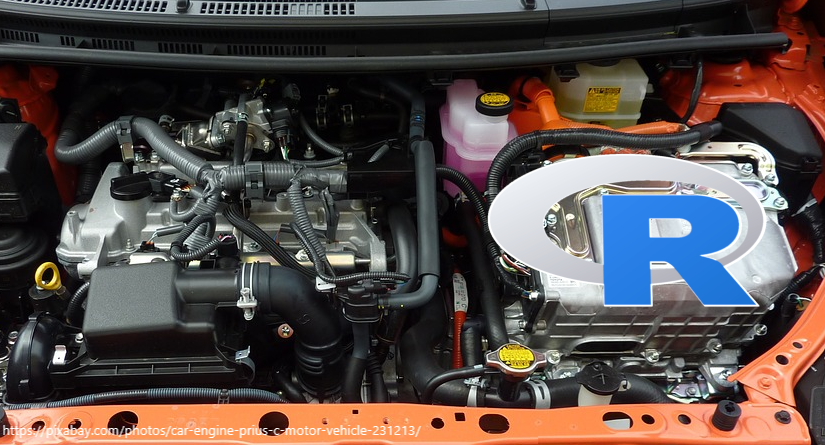
\includegraphics[width=2.08333in,height=\textheight]{././pic/101_engine_R.png}
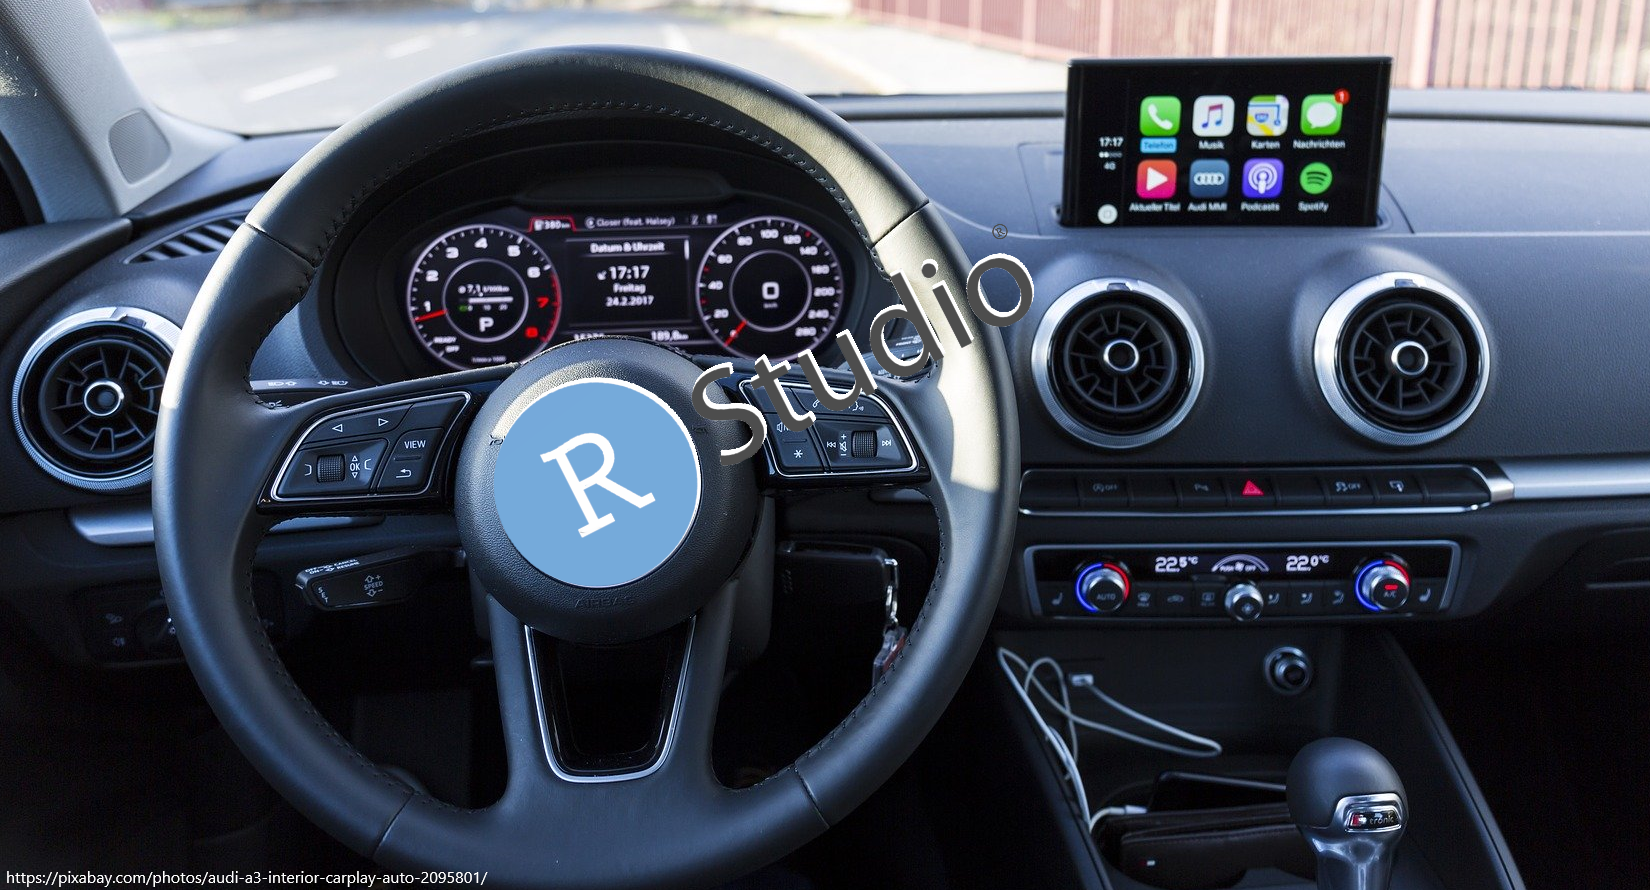
\includegraphics[width=2.08333in,height=\textheight]{././pic/101_cockpit_rstudio2.png}

}

}

\end{minipage}%

\caption{\label{fig-rstudio}R und RStudio}

\end{figure}

\hypertarget{rstudio-einrichten}{%
\section{RStudio einrichten}\label{rstudio-einrichten}}

Öffnen Sie nach erfolgreicher Installation die Anwendung RStudio

\includegraphics[width=0.20833in,height=\textheight]{././pic/rstudio-icon.png}
und Sie sollten folgende Ansicht vor sich sehen:

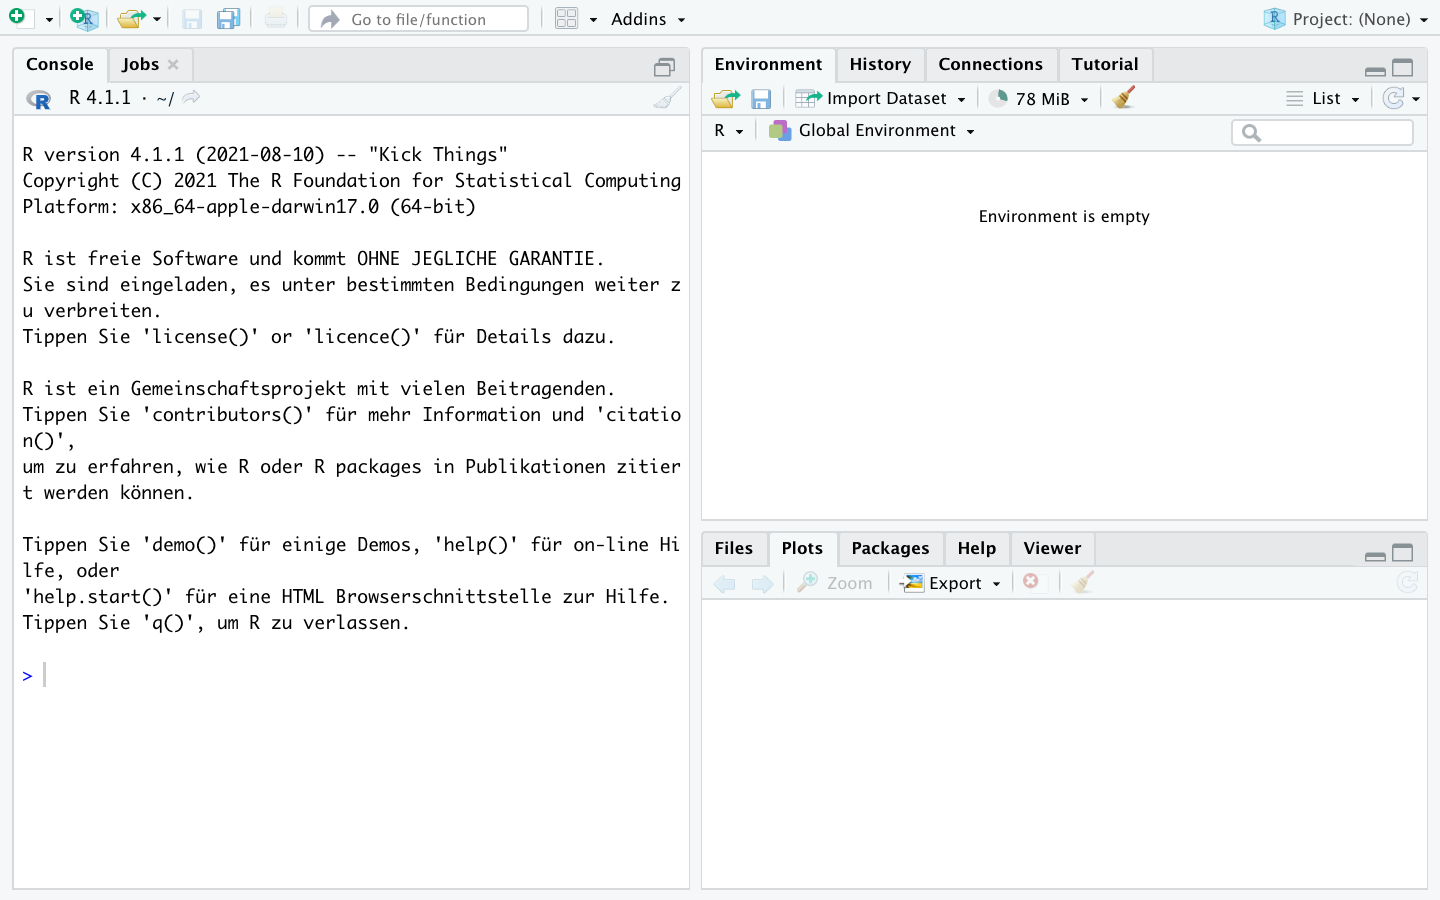
\includegraphics{././pic/101_RStudio.png}

Um Probleme bei der künftigen Arbeit mit R zu vermeiden, deaktivieren
Sie bitte das automatische Speichern und Laden des Workspace. Rufen Sie
dazu das entsprechende Menü unter dem Reiter ``Tools -\textgreater{}
Global options'' auf und deaktivieren Sie bitte ``Restore .RData into
workspace at startup'' und setzen Sie ``Save workspace to .RData on
exit:'' auf \texttt{Never}. RStudio speichert ansonsten alle geladenen
Objekte wenn Sie die Sitzung beenden und lädt diese automatisch wenn Sie
das Programm das nächste Mal öffnen. Dies führt erfahrungsgemäß zu
Problemen.

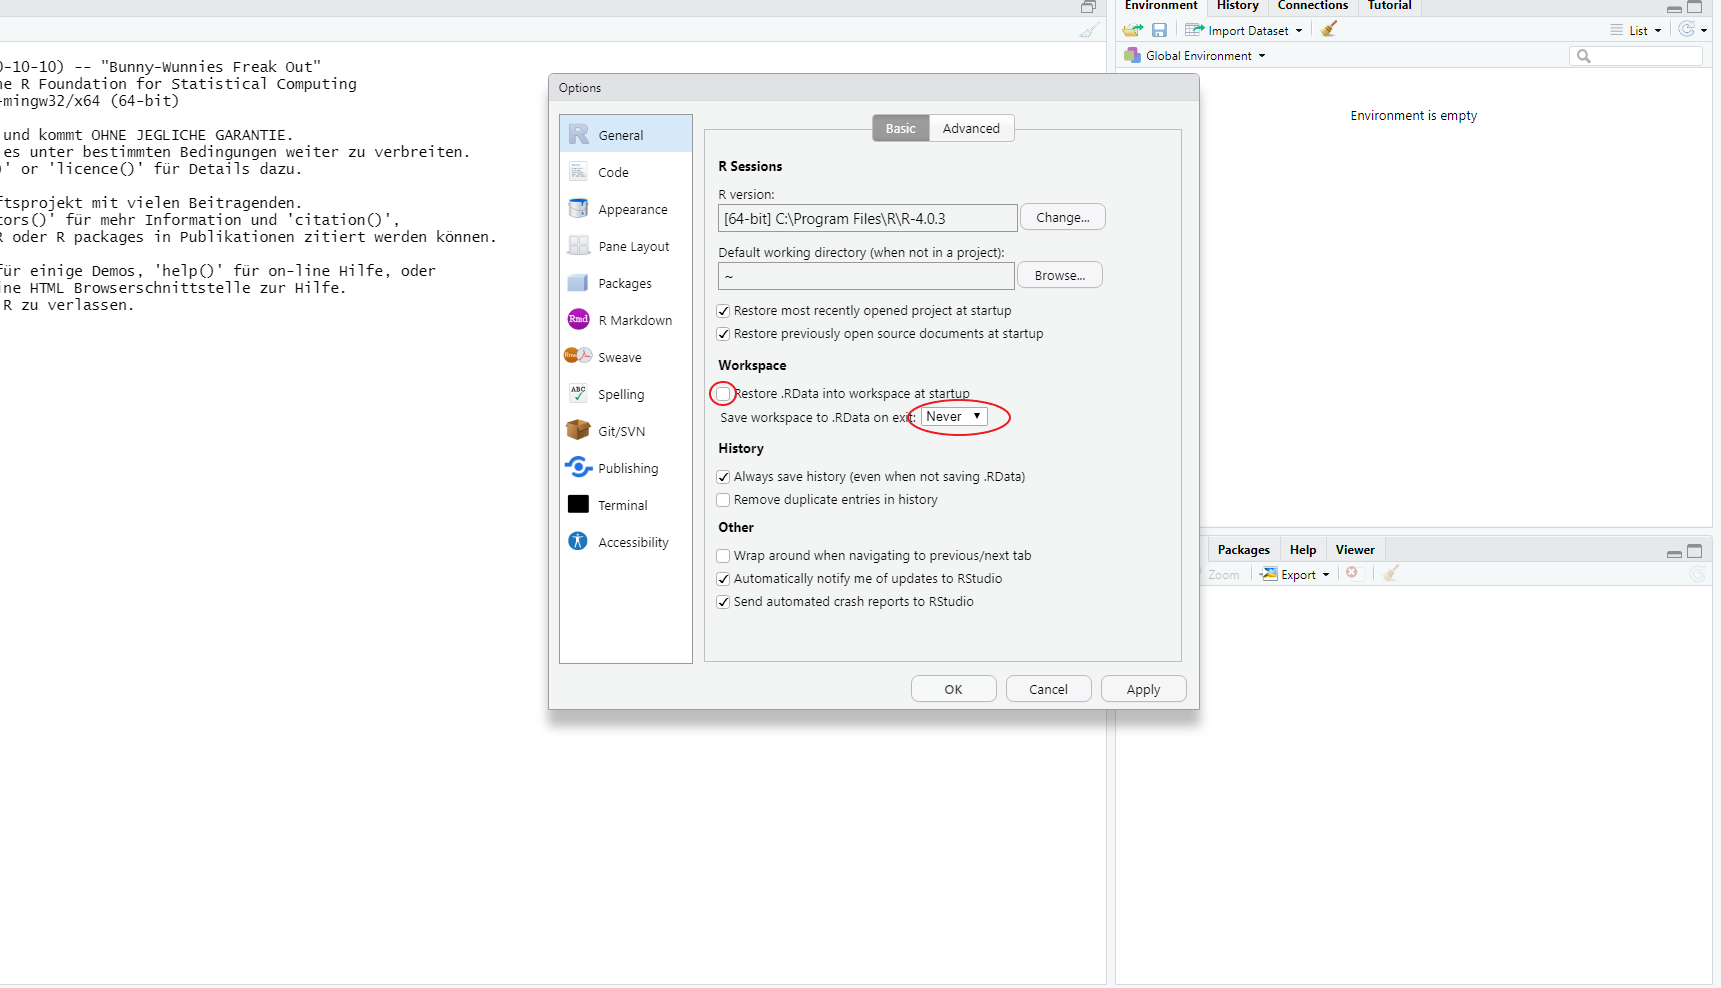
\includegraphics{././pic/101_RStudio_setup.png}

Bestätigen Sie die Einstellungen mit ``Apply'' und schließen Sie das
Fenster mit ``OK''.

\hypertarget{erste-schritte-in-r}{%
\section{Erste Schritte in R}\label{erste-schritte-in-r}}

Nach diesen grundlegenden Einstellungen können wir uns an die ersten
Schritte in R machen. Öffnen Sie dazu zunächst ein Script, indem Sie auf
das weiße Symbol links oben klicken oder drücken Sie gleichzeitig
STRG/Command + Shift + N .

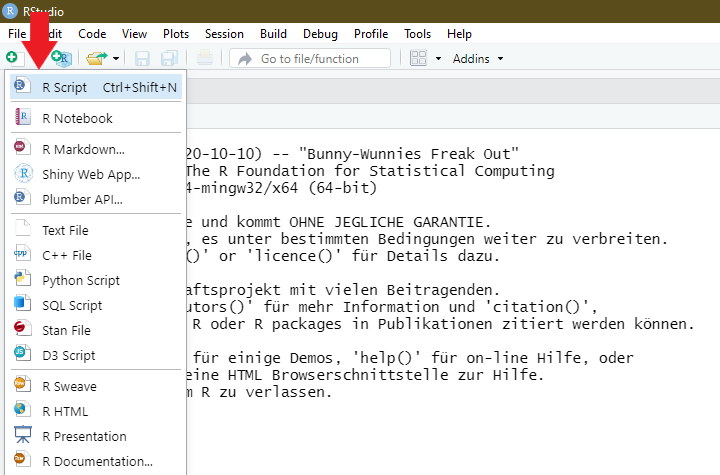
\includegraphics[width=4.5625in,height=\textheight]{././pic/101_RStudio_script2.png}

Es öffnet sich ein viertes Fenster, sodass Sie nun folgende Ansicht vor
sich haben sollten:

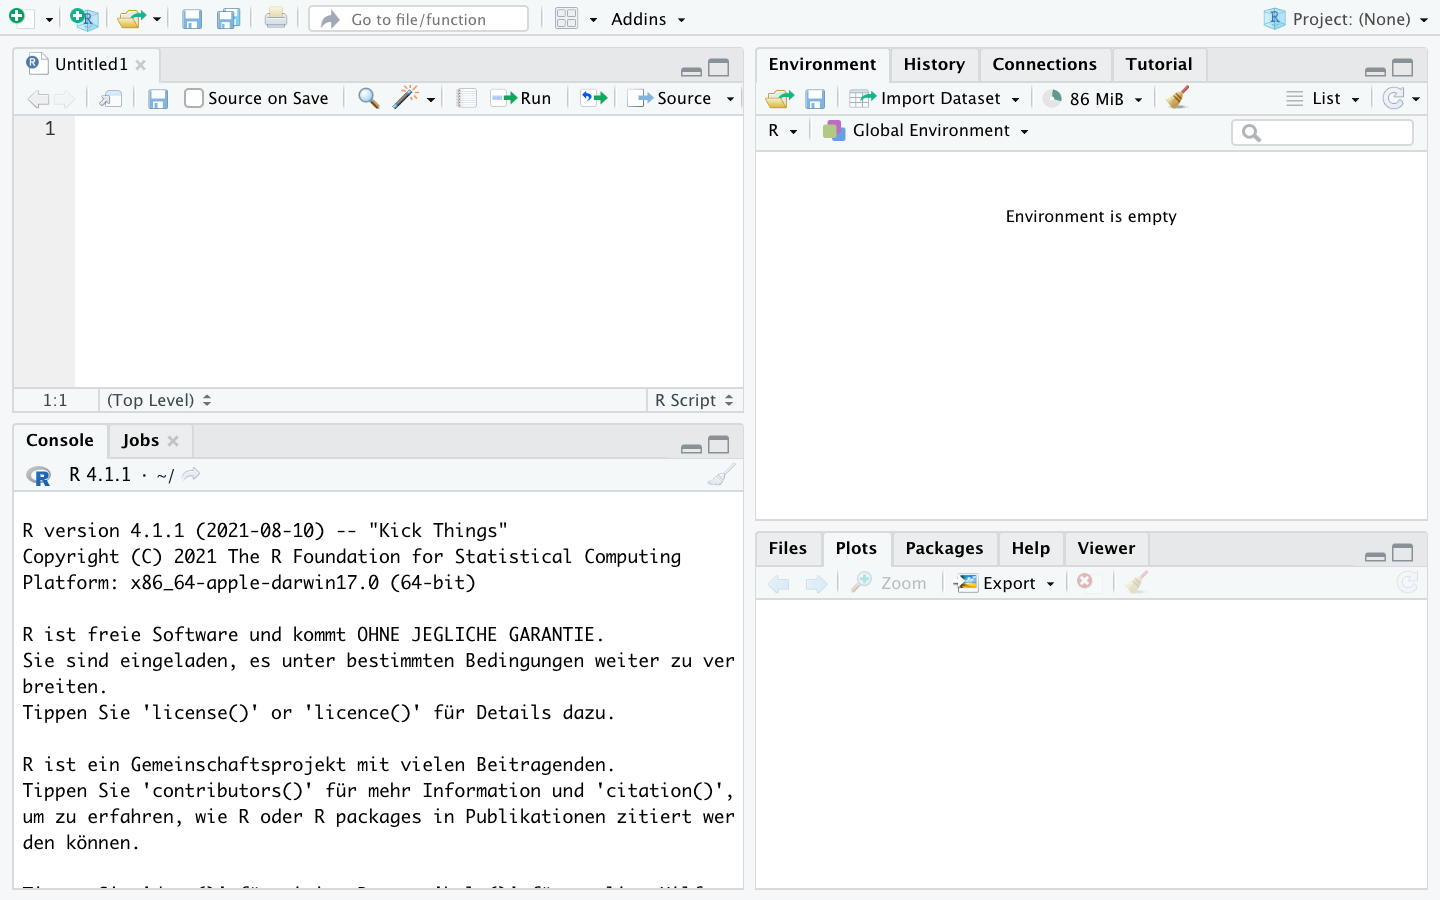
\includegraphics{././pic/101_RStudio_script.png}

Dieser Scripteditor ist der Ort, an dem wir Befehle erstellen und
anschließend durchführen werden. Der Scripteditor dient dabei als
Sammlung aller durchzuführenden Befehle. Wir können diese Sammlungen
speichern, um sie später wieder aufzurufen und vor allem können wir so
Befehlssammlungen mit anderen teilen oder Skripte von anderen für uns
selbst nutzen. Wir entwerfen also zunächst im Scripteditor eine
Rechnung:

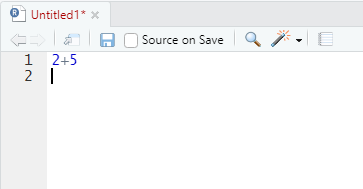
\includegraphics[width=3.54167in,height=\textheight]{././pic/101_RStudio_script0.png}

Um diese nun auszuführen, klicken wir in die auszuführende Zeile, sodass
der Cursor in dieser Zeile ist und drücken gleichzeitig STRG und Enter
(Mac-User Command und Enter):

\begin{figure}

\begin{minipage}[t]{0.50\linewidth}

{\centering 

\raisebox{-\height}{

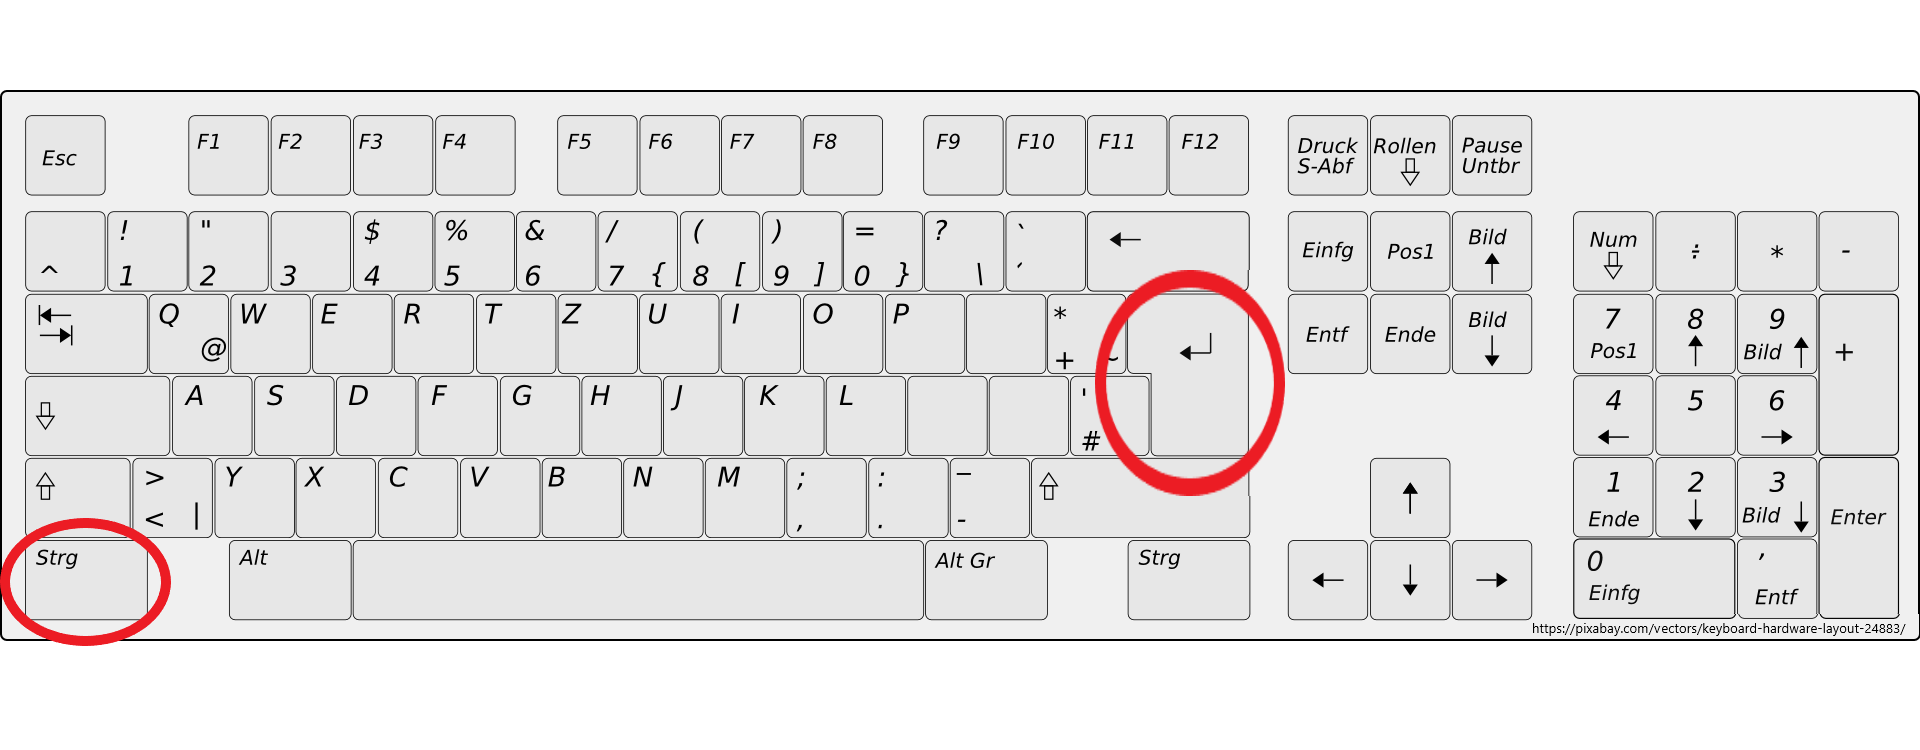
\includegraphics[width=4.0625in,height=\textheight]{././pic/101_keyboard_pc.png}

}

}

\end{minipage}%
%
\begin{minipage}[t]{0.50\linewidth}

{\centering 

\raisebox{-\height}{

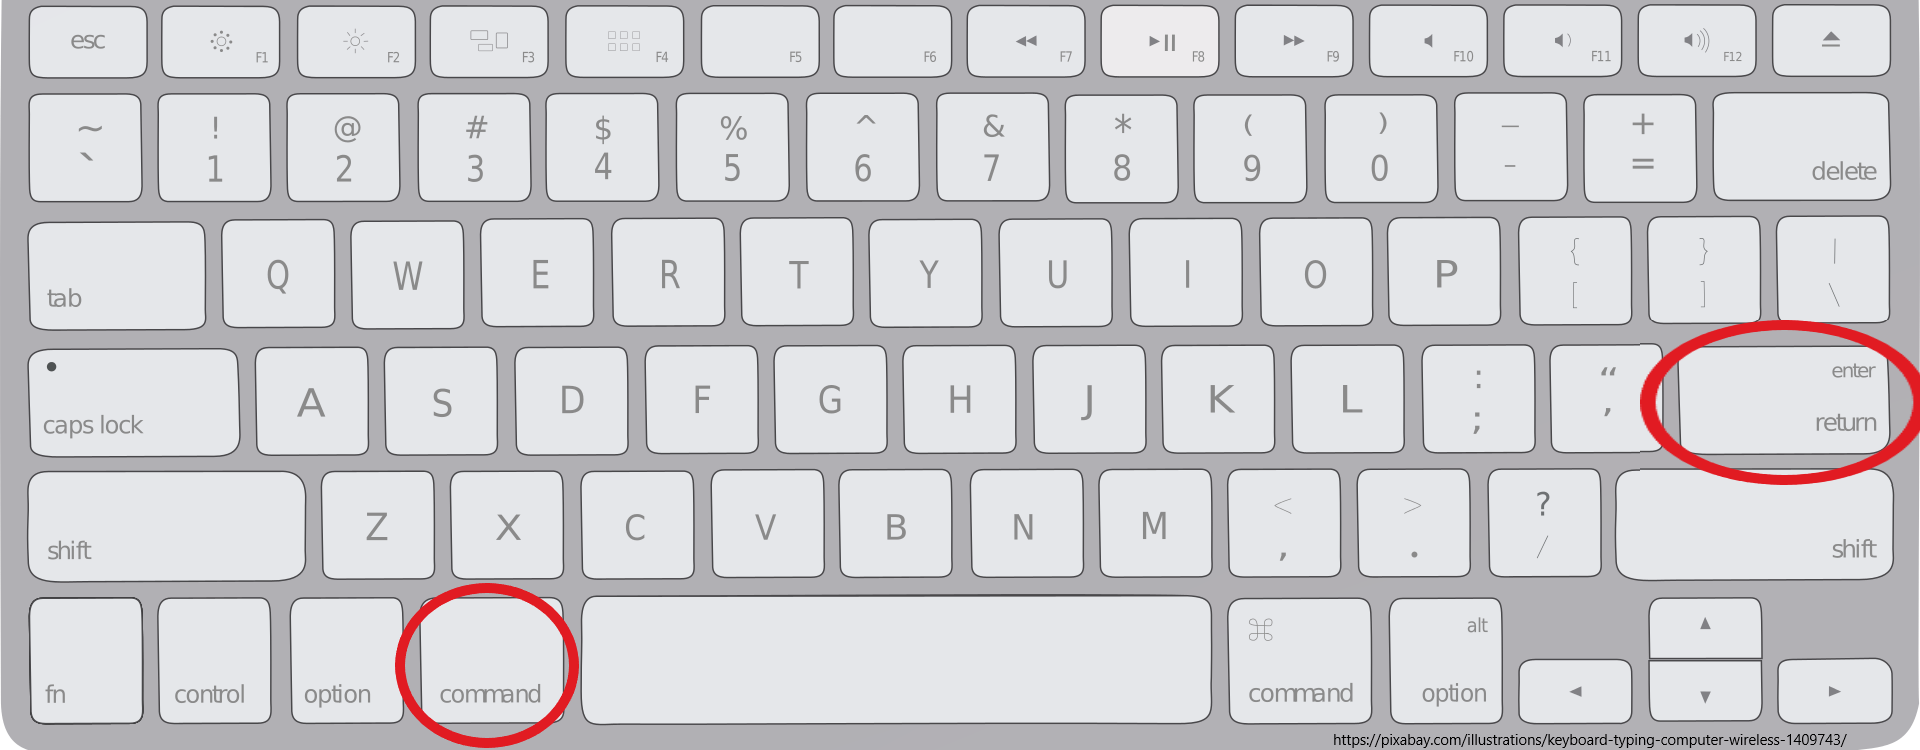
\includegraphics[width=4.0625in,height=\textheight]{././pic/101_keyboard_mac.png}

}

}

\end{minipage}%

\caption{\label{fig-keys}Shortcuts für Berechnungen}

\end{figure}

R gibt die Ergebnisse unten in der Console aus:

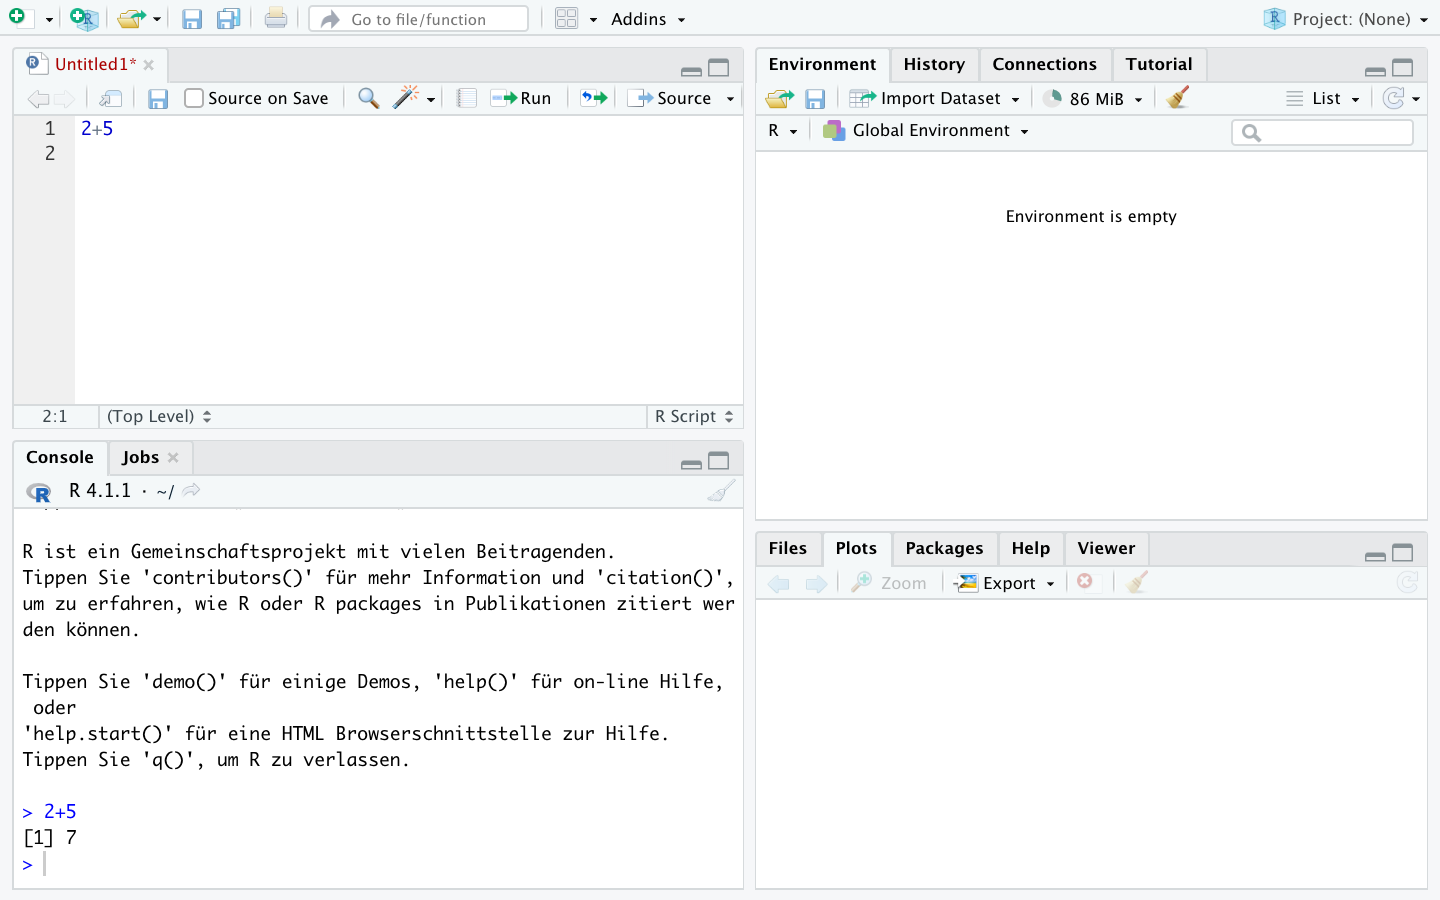
\includegraphics{././pic/101_RStudio_Erste_Rechnung.png}

Das funktioniert auch für mehrere Rechnungen auf einmal indem wir
mehrere Zeilen markieren und dann wieder STRG und Enter (Mac-User
Command und Enter) drücken:

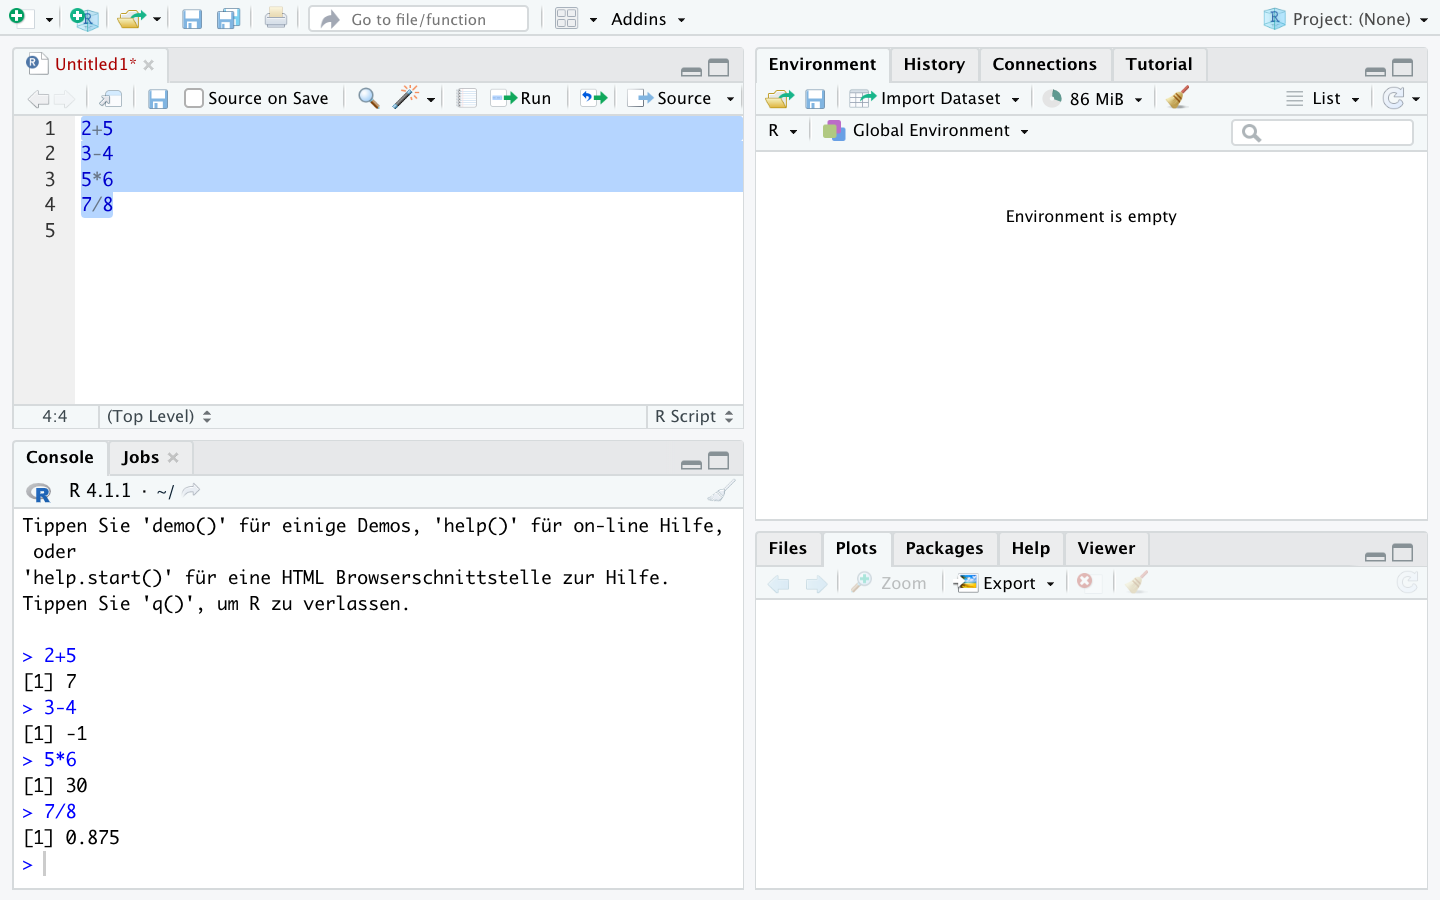
\includegraphics{././pic/101_RStudio_Rechnung.png}

Eingaben aus dem Script-Editor und Ergebnisse aus der Konsole werden in
Zukunft so dargestellt:

\begin{Shaded}
\begin{Highlighting}[]
\DecValTok{2}\SpecialCharTok{+}\DecValTok{5}
\end{Highlighting}
\end{Shaded}

\begin{verbatim}
[1] 7
\end{verbatim}

\begin{Shaded}
\begin{Highlighting}[]
\DecValTok{3{-}4}
\end{Highlighting}
\end{Shaded}

\begin{verbatim}
[1] -1
\end{verbatim}

\begin{Shaded}
\begin{Highlighting}[]
\DecValTok{5}\SpecialCharTok{*}\DecValTok{6}
\end{Highlighting}
\end{Shaded}

\begin{verbatim}
[1] 30
\end{verbatim}

\begin{Shaded}
\begin{Highlighting}[]
\DecValTok{7}\SpecialCharTok{/}\DecValTok{8}
\end{Highlighting}
\end{Shaded}

\begin{verbatim}
[1] 0.875
\end{verbatim}

R beherrscht natürlich auch längere Berechnungen, zum Beispiel wird auch
Punkt vor Strich beachtet:

\begin{Shaded}
\begin{Highlighting}[]
\DecValTok{2}\SpecialCharTok{+}\DecValTok{3}\SpecialCharTok{*}\DecValTok{2}
\end{Highlighting}
\end{Shaded}

\begin{verbatim}
[1] 8
\end{verbatim}

\begin{Shaded}
\begin{Highlighting}[]
\NormalTok{(}\DecValTok{2}\SpecialCharTok{+}\DecValTok{3}\NormalTok{)}\SpecialCharTok{*}\DecValTok{2}
\end{Highlighting}
\end{Shaded}

\begin{verbatim}
[1] 10
\end{verbatim}

Auch weitere Operationen sind möglich:

\begin{Shaded}
\begin{Highlighting}[]
\DecValTok{4}\SpecialCharTok{\^{}}\DecValTok{2} \DocumentationTok{\#\# 4²}
\end{Highlighting}
\end{Shaded}

\begin{verbatim}
[1] 16
\end{verbatim}

\begin{Shaded}
\begin{Highlighting}[]
\FunctionTok{sqrt}\NormalTok{(}\DecValTok{4}\NormalTok{) }\DocumentationTok{\#\# Wurzel }
\end{Highlighting}
\end{Shaded}

\begin{verbatim}
[1] 2
\end{verbatim}

\begin{Shaded}
\begin{Highlighting}[]
\FunctionTok{exp}\NormalTok{(}\DecValTok{1}\NormalTok{) }\DocumentationTok{\#\# Exponentialfunktion (Eulersche Zahl)}
\end{Highlighting}
\end{Shaded}

\begin{verbatim}
[1] 2.718282
\end{verbatim}

\begin{Shaded}
\begin{Highlighting}[]
\FunctionTok{log}\NormalTok{(}\DecValTok{5}\NormalTok{) }\DocumentationTok{\#\# Natürlicher Logarithmus}
\end{Highlighting}
\end{Shaded}

\begin{verbatim}
[1] 1.609438
\end{verbatim}

\begin{Shaded}
\begin{Highlighting}[]
\FunctionTok{log}\NormalTok{(}\FunctionTok{exp}\NormalTok{(}\DecValTok{5}\NormalTok{)) }\DocumentationTok{\#\# log und exp heben sich gegenseitig auf}
\end{Highlighting}
\end{Shaded}

\begin{verbatim}
[1] 5
\end{verbatim}

Ergebnisse lassen sich mit einem \texttt{\textless{}-} unter einem
beliebigen Namen als Objekt speichern. Dann wird R uns nicht das
Ergebnis anzeigen, sondern den Befehl in der Konsole wiederholen:

\begin{Shaded}
\begin{Highlighting}[]
\NormalTok{x }\OtherTok{\textless{}{-}} \DecValTok{4}\SpecialCharTok{/}\DecValTok{2}
\end{Highlighting}
\end{Shaded}

Im Fenster ``Environment'' rechts oben sehen wir jetzt das abgelegte
Objekt \texttt{x}:

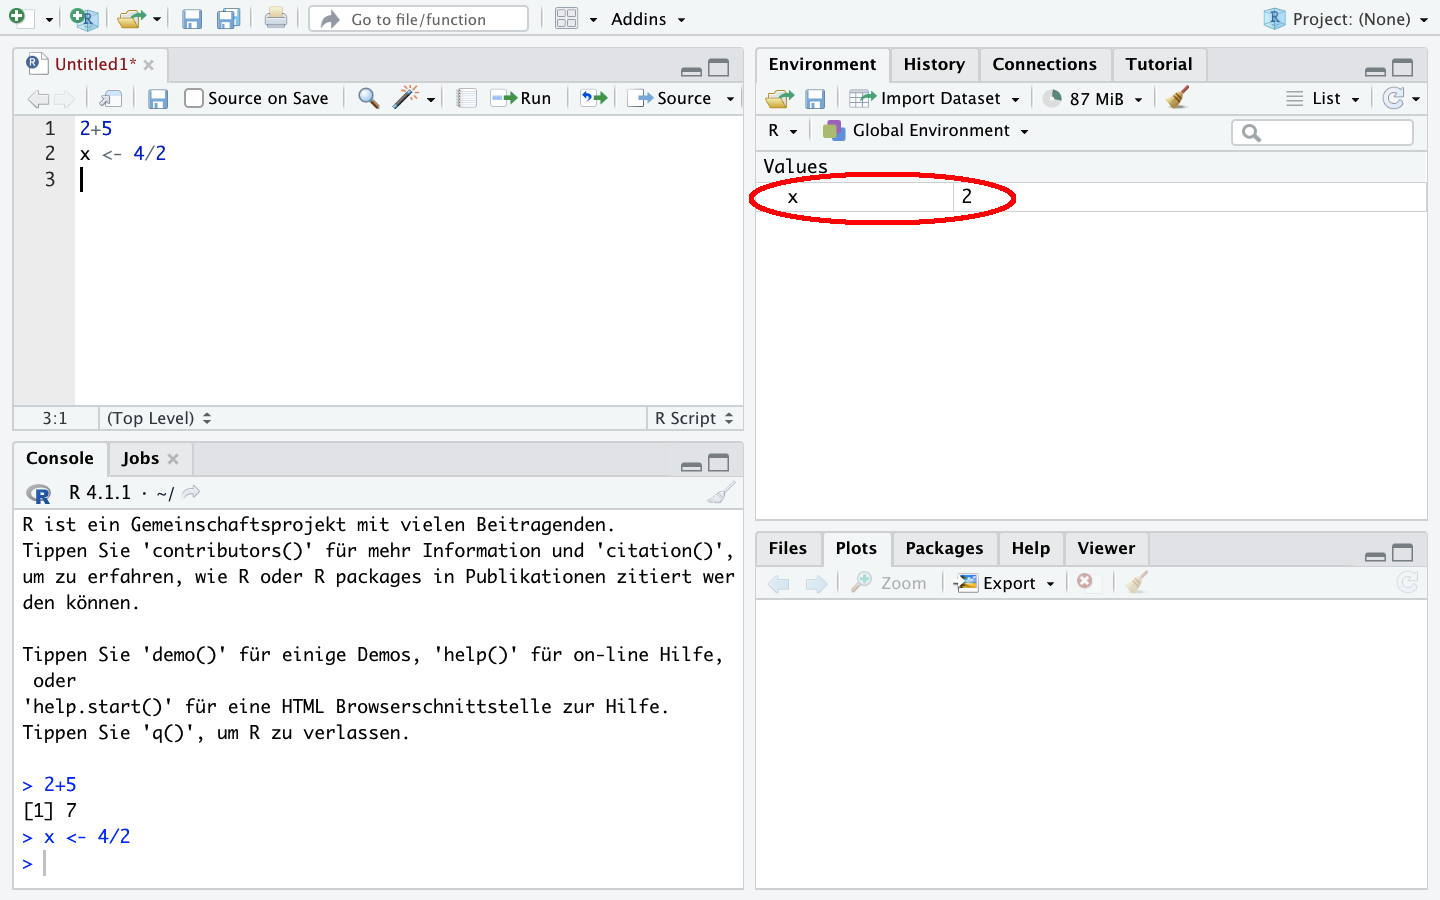
\includegraphics{././pic/101_RStudio_Environment2.png}

Wir können es später wieder aufrufen:

\begin{Shaded}
\begin{Highlighting}[]
\NormalTok{x}
\end{Highlighting}
\end{Shaded}

\begin{verbatim}
[1] 2
\end{verbatim}

Außerdem können wir Objekte in Rechnungen weiter verwenden - wir setzen
einfach \texttt{x} ein und erstellen zB. \texttt{y}:

\begin{Shaded}
\begin{Highlighting}[]
\NormalTok{y }\OtherTok{\textless{}{-}}\NormalTok{ x }\SpecialCharTok{*} \DecValTok{5}
\NormalTok{y}
\end{Highlighting}
\end{Shaded}

\begin{verbatim}
[1] 10
\end{verbatim}

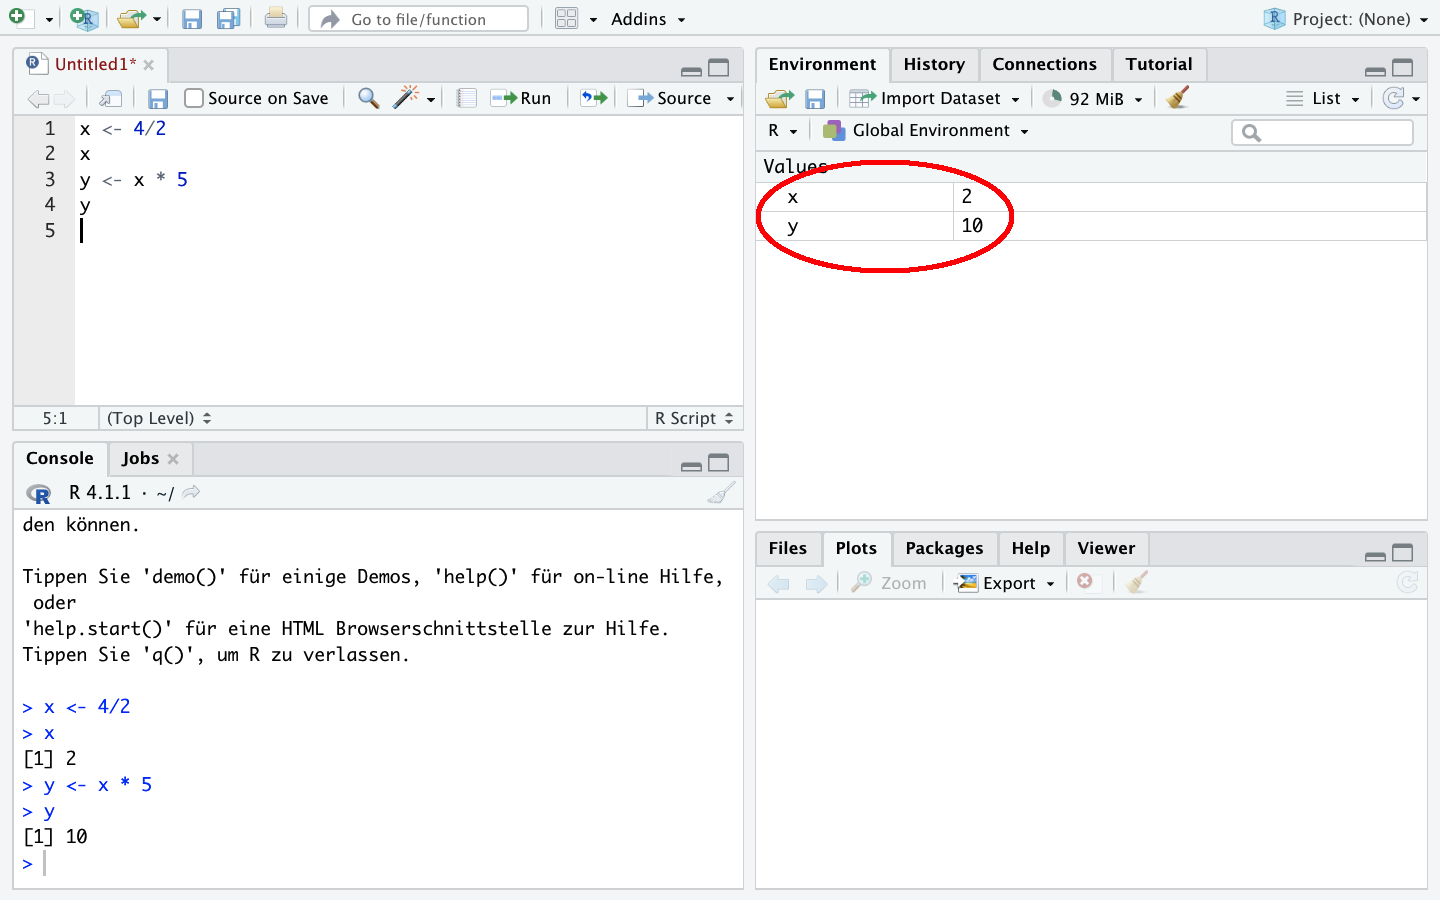
\includegraphics{././pic/101_RStudio_Environment.png}

Mit \texttt{c()} lassen sich mehrere Werte unter einem Objekt ablegen
und auch mit diesen lässt sich rechnen:

\begin{Shaded}
\begin{Highlighting}[]
\NormalTok{x1 }\OtherTok{\textless{}{-}} \FunctionTok{c}\NormalTok{(}\DecValTok{1}\NormalTok{,}\DecValTok{2}\NormalTok{,}\DecValTok{3}\NormalTok{)}
\NormalTok{x1}
\end{Highlighting}
\end{Shaded}

\begin{verbatim}
[1] 1 2 3
\end{verbatim}

\begin{Shaded}
\begin{Highlighting}[]
\NormalTok{x1}\SpecialCharTok{*} \DecValTok{2}
\end{Highlighting}
\end{Shaded}

\begin{verbatim}
[1] 2 4 6
\end{verbatim}

\begin{Shaded}
\begin{Highlighting}[]
\NormalTok{y1 }\OtherTok{\textless{}{-}} \FunctionTok{c}\NormalTok{(}\DecValTok{10}\NormalTok{,}\DecValTok{11}\NormalTok{,}\DecValTok{9}\NormalTok{)}
\NormalTok{y1}
\end{Highlighting}
\end{Shaded}

\begin{verbatim}
[1] 10 11  9
\end{verbatim}

\begin{Shaded}
\begin{Highlighting}[]
\NormalTok{y1}\SpecialCharTok{/}\NormalTok{x1}
\end{Highlighting}
\end{Shaded}

\begin{verbatim}
[1] 10.0  5.5  3.0
\end{verbatim}

Natürlich können wir Objekte auch wieder löschen und zwar mit
\texttt{rm()}. Wenn wir ein nicht existierendes Objekt aufrufen bekommen
wir eine Fehlermeldung:

\begin{Shaded}
\begin{Highlighting}[]
\FunctionTok{rm}\NormalTok{(x1)}
\NormalTok{x1}
\end{Highlighting}
\end{Shaded}

\begin{verbatim}
Error in eval(expr, envir, enclos): Objekt 'x1' nicht gefunden
\end{verbatim}

Mit \texttt{rm(list\ =\ ls())} können alle Objekte aus dem Environment
gelöscht werden.

Das Script können wir speichern, um es später wieder aufzurufen.

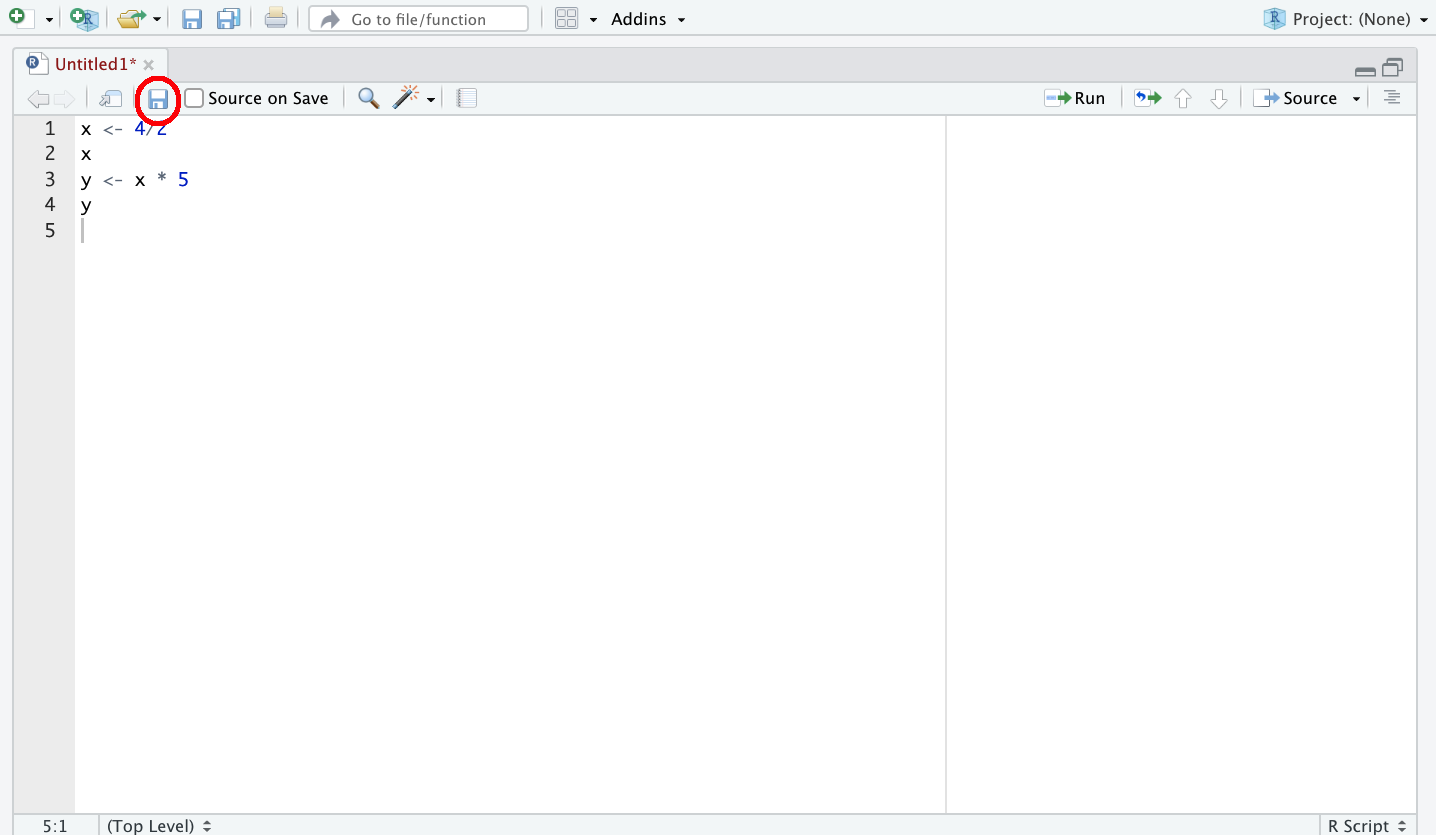
\includegraphics[width=3.5625in,height=\textheight]{././pic/101_RStudio_script3.png}

Wichtig ist dabei, der gespeicherten Datei die Endung ``.R'' zu geben,
also zum Beispiel ``R\_Script1.R''.

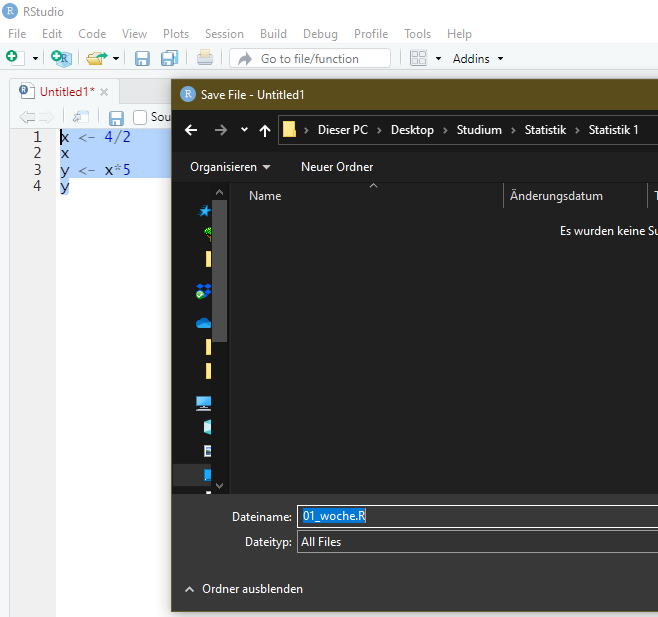
\includegraphics[width=3.22917in,height=\textheight]{././pic/101_RStudio_script4.png}

\textbf{Tipp:} Erstellen Sie sich am besten sofort einen Ordner, in dem
Sie alle R Scripte und Datensätze\footnote{Was das ist, werden wir in
  der kommenden Session lernen.} aus dieser Veranstaltung gesammelt
ablegen.

\hypertarget{aufgaben}{%
\section{Aufgaben}\label{aufgaben}}

\begin{itemize}
\item
  Berechnen Sie das aktuelle Alter einer Person, die im Jahr 1977
  geboren wurde!
\item
  Legen Sie das Ergebnis unter \texttt{age} ab.
\item
  Wie können Sie \texttt{age} aufrufen, um zu sehen welcher Wert
  abgelegt wurde?
\item
  Legen Sie die Anzahl der Studierenden an der Uni Oldenburg (15643)
  unter \texttt{stud} ab.
\item
  Legen Sie die Anzahl der Professuren an der Uni Oldenburg (210) unter
  \texttt{prof} ab.
\item
  Berechnen Sie die Anzahl der Studierenden pro Professur an der Uni
  Oldenburg indem Sie die Objekte \texttt{stud} und \texttt{prof}
  verwenden.
\item
  Legen Sie das Ergebnis unter \texttt{studprof} ab und rufen Sie das
  das Objekt noch einmal auf!
\item
  Sehen Sie die erstellten Variablen im Environment-Fenster?
\item
  Löschen Sie das Objekt \texttt{stud}. Woran erkennen Sie, dass das
  funktioniert hat?
\item
  Legen Sie die Studierendenzahlen der Uni Bremen (19173), Uni Vechta
  (5333) und Uni Oldenburg (15643) zusammen unter \texttt{studs} ab.
\item
  Legen Sie die Zahl der Profs der Uni Bremen (322), Uni Vechta (67) und
  Uni Oldenburg (210) zusammen unter \texttt{profs} ab.
\item
  Berechnen die Anzahl der Studierenden pro Professur für alle drei
  Universitäten.
\item
  Sie möchten zusätzlich die Zahl der Studierenden (14000) und
  Professuren (217) der Uni Osnabrück in \texttt{studs} und
  \texttt{profs} ablegen. Wie gehen Sie vor?
\item
  Berechnen Sie für alle vier Universitäten das Verhältnis von
  Studierenden und Professuren!
\item
  Löschen Sie alle Objekte aus dem Environment.
\end{itemize}

In der ersten Session haben wir ein paar erste Schritte mit der
Taschenrechnerfunktion in R unternommen. Die wirkliche Stärke von R ist
aber die Verarbeitung von Daten - das lernen wir heute kennen.

Im vorherigen Kapitel haben wir die Studierendenzahlen der Uni Bremen
(19173), Uni Vechta (5333) und Uni Oldenburg (15643) zusammen unter
\texttt{studs} abgelegt und mit den in \texttt{profs} abgelegten
Professurenzahlen ins Verhältnis gesetzt. Das funktioniert soweit gut,
allerdings ist es übersichtlicher, zusammengehörige Werte auch zusammen
ablegen. Dafür gibt es in R \texttt{data.frame}. Wir können dazu die
beiden Objekte in einem Datensatz ablegen, indem wir sie in
\texttt{data.frame} eintragen und das neue Objekt unter \texttt{df}
ablegen. Wenn wir \texttt{df} aufrufen sehen wir, dass die Werte
zeilenweise zusammengefügt wurden:

\begin{Shaded}
\begin{Highlighting}[]
\NormalTok{studs }\OtherTok{\textless{}{-}} \FunctionTok{c}\NormalTok{(}\DecValTok{19173}\NormalTok{,}\DecValTok{5333}\NormalTok{,}\DecValTok{15643}\NormalTok{)    }\DocumentationTok{\#\# Studierendenzahlen unter "studs" ablegen }
\NormalTok{profs       }\OtherTok{\textless{}{-}} \FunctionTok{c}\NormalTok{(}\DecValTok{322}\NormalTok{,}\DecValTok{67}\NormalTok{,}\DecValTok{210}\NormalTok{)    }\DocumentationTok{\#\# Prof{-}Zahlen unter "profs" ablegen}
\NormalTok{df }\OtherTok{\textless{}{-}} \FunctionTok{data.frame}\NormalTok{(studs, profs)}
\NormalTok{df    }\DocumentationTok{\#\# zeigt den kompletten Datensatz an}
\end{Highlighting}
\end{Shaded}

\begin{verbatim}
  studs profs
1 19173   322
2  5333    67
3 15643   210
\end{verbatim}

In der ersten Zeile stehen also die Werte der Uni Bremen, in der zweiten
Zeile die Werte der Uni Vechta usw. Die Werte können wir dann mit
\texttt{datensatzname\$variablenname} aufrufen. So können wir die Spalte
\texttt{profs} anzeigen lassen:

\begin{Shaded}
\begin{Highlighting}[]
\NormalTok{df}\SpecialCharTok{$}\NormalTok{profs }
\end{Highlighting}
\end{Shaded}

\begin{verbatim}
[1] 322  67 210
\end{verbatim}

Mit \texttt{colnames()} können wir die Variablen-/Spaltennamen des
Datensatzes anzeigen lassen, zudem können wir mit \texttt{nrow} und
\texttt{ncol} die Zahl der Zeilen bzw. Spalten aufrufen:

\begin{Shaded}
\begin{Highlighting}[]
\FunctionTok{colnames}\NormalTok{(df) }\DocumentationTok{\#\# Variablen{-}/Spaltennamen anzeigen}
\end{Highlighting}
\end{Shaded}

\begin{verbatim}
[1] "studs" "profs"
\end{verbatim}

\begin{Shaded}
\begin{Highlighting}[]
\FunctionTok{ncol}\NormalTok{(df) }\DocumentationTok{\#\# Anzahl der Spalten/Variablen}
\end{Highlighting}
\end{Shaded}

\begin{verbatim}
[1] 2
\end{verbatim}

\begin{Shaded}
\begin{Highlighting}[]
\FunctionTok{nrow}\NormalTok{(df) }\DocumentationTok{\#\# Anzahl der Zeilen/Fälle}
\end{Highlighting}
\end{Shaded}

\begin{verbatim}
[1] 3
\end{verbatim}

Neue zusätzliche Variablen können durch
\texttt{datensatzname\$neuevariable} in den Datensatz eingefügt werden:

\begin{Shaded}
\begin{Highlighting}[]
\NormalTok{df}\SpecialCharTok{$}\NormalTok{stu\_prof }\OtherTok{\textless{}{-}}\NormalTok{ df}\SpecialCharTok{$}\NormalTok{studs}\SpecialCharTok{/}\NormalTok{df}\SpecialCharTok{$}\NormalTok{profs}
\DocumentationTok{\#\# df hat also nun eine Spalte mehr:}
\FunctionTok{ncol}\NormalTok{(df) }
\end{Highlighting}
\end{Shaded}

\begin{verbatim}
[1] 3
\end{verbatim}

\begin{Shaded}
\begin{Highlighting}[]
\NormalTok{df}
\end{Highlighting}
\end{Shaded}

\begin{verbatim}
  studs profs stu_prof
1 19173   322 59.54348
2  5333    67 79.59701
3 15643   210 74.49048
\end{verbatim}

\hypertarget{variablentypen}{%
\section{Variablentypen}\label{variablentypen}}

Wir können auch ein oder mehrere Wörter in einer Variable ablegen,
jedoch müssen Buchstaben/Wörter immer in \texttt{""} gesetzt werden.

\begin{Shaded}
\begin{Highlighting}[]
\NormalTok{df}\SpecialCharTok{$}\NormalTok{uni }\OtherTok{\textless{}{-}} \FunctionTok{c}\NormalTok{(}\StringTok{"Uni Bremen"}\NormalTok{,}\StringTok{"Uni Vechta"}\NormalTok{, }\StringTok{"Uni Oldenburg"}\NormalTok{)}
\NormalTok{df}
\end{Highlighting}
\end{Shaded}

\begin{verbatim}
  studs profs stu_prof           uni
1 19173   322 59.54348    Uni Bremen
2  5333    67 79.59701    Uni Vechta
3 15643   210 74.49048 Uni Oldenburg
\end{verbatim}

Damit haben wir einen neuen Variablentypen kennen gelernt. Grundsätzlich
gibt es in R zwei Variablentypen: numeric (enthält Zahlen) und character
(enthält Text oder Zahlen, die als Text verstanden werden sollen).
Darüber hinaus gibt es noch weitere Typen, die besprechen wir wenn sie
nötig sind, zB. gibt es ``integer'' für numerische Variablen mit
ausschließlich ganzzahligen Ausprägungen. Mit \texttt{class()} kann die
Art der Variable untersucht werden oder mit \texttt{is.numeric()} bzw.
\texttt{is.character()} können wir abfragen ob eine Variable diesem Typ
entspricht:

\begin{Shaded}
\begin{Highlighting}[]
\FunctionTok{class}\NormalTok{(df}\SpecialCharTok{$}\NormalTok{profs)}
\end{Highlighting}
\end{Shaded}

\begin{verbatim}
[1] "numeric"
\end{verbatim}

\begin{Shaded}
\begin{Highlighting}[]
\FunctionTok{class}\NormalTok{(df}\SpecialCharTok{$}\NormalTok{uni)}
\end{Highlighting}
\end{Shaded}

\begin{verbatim}
[1] "character"
\end{verbatim}

\begin{Shaded}
\begin{Highlighting}[]
\FunctionTok{is.numeric}\NormalTok{(df}\SpecialCharTok{$}\NormalTok{profs)}
\end{Highlighting}
\end{Shaded}

\begin{verbatim}
[1] TRUE
\end{verbatim}

\begin{Shaded}
\begin{Highlighting}[]
\FunctionTok{is.numeric}\NormalTok{(df}\SpecialCharTok{$}\NormalTok{uni)}
\end{Highlighting}
\end{Shaded}

\begin{verbatim}
[1] FALSE
\end{verbatim}

\begin{Shaded}
\begin{Highlighting}[]
\FunctionTok{is.character}\NormalTok{(df}\SpecialCharTok{$}\NormalTok{profs)}
\end{Highlighting}
\end{Shaded}

\begin{verbatim}
[1] FALSE
\end{verbatim}

Mit \texttt{as.character()} bzw. \texttt{as.numeric()} können wir einen
Typenwechsel erzwingen:

\begin{Shaded}
\begin{Highlighting}[]
\FunctionTok{as.character}\NormalTok{(df}\SpecialCharTok{$}\NormalTok{profs) }\DocumentationTok{\#\# die "" zeigen an, dass die Variable als character definiert ist}
\end{Highlighting}
\end{Shaded}

\begin{verbatim}
[1] "322" "67"  "210"
\end{verbatim}

Das ändert erstmal nichts an der Ausgangsvariable \texttt{df\$profs}:

\begin{Shaded}
\begin{Highlighting}[]
\FunctionTok{class}\NormalTok{(df}\SpecialCharTok{$}\NormalTok{profs)}
\end{Highlighting}
\end{Shaded}

\begin{verbatim}
[1] "numeric"
\end{verbatim}

Wir können diese Umwandlung auch permanent machen, indem wir
\texttt{df\$profs} mit der umgewandelten Variante überschreiben:

\begin{Shaded}
\begin{Highlighting}[]
\NormalTok{df}\SpecialCharTok{$}\NormalTok{profs }\OtherTok{\textless{}{-}} \FunctionTok{as.character}\NormalTok{(df}\SpecialCharTok{$}\NormalTok{profs)}
\NormalTok{df}\SpecialCharTok{$}\NormalTok{profs }
\end{Highlighting}
\end{Shaded}

\begin{verbatim}
[1] "322" "67"  "210"
\end{verbatim}

\begin{Shaded}
\begin{Highlighting}[]
\FunctionTok{class}\NormalTok{(df}\SpecialCharTok{$}\NormalTok{profs)}
\end{Highlighting}
\end{Shaded}

\begin{verbatim}
[1] "character"
\end{verbatim}

Mit \texttt{character}-Variablen kann nicht gerechnet werden, auch wenn
sie Zahlen enthalten:

\begin{Shaded}
\begin{Highlighting}[]
\NormalTok{df}\SpecialCharTok{$}\NormalTok{profs }\SpecialCharTok{/} \DecValTok{2} 
\end{Highlighting}
\end{Shaded}

\begin{verbatim}
Error in df$profs/2: nicht-numerisches Argument für binären Operator
\end{verbatim}

Wir können aber natürlich \texttt{df\$profs} spontan in \texttt{numeric}
umwandeln, um mit den Zahlenwerten zu rechnen:

\begin{Shaded}
\begin{Highlighting}[]
\FunctionTok{as.numeric}\NormalTok{(df}\SpecialCharTok{$}\NormalTok{profs) }\SpecialCharTok{/} \DecValTok{2}
\end{Highlighting}
\end{Shaded}

\begin{verbatim}
[1] 161.0  33.5 105.0
\end{verbatim}

Wenn wir Textvariablen in numerische Variablen umwandeln, bekommen wir
\texttt{NA}s ausgegeben. \texttt{NA} steht in R für fehlende Werte:

\begin{Shaded}
\begin{Highlighting}[]
\FunctionTok{as.numeric}\NormalTok{(df}\SpecialCharTok{$}\NormalTok{uni)}
\end{Highlighting}
\end{Shaded}

\begin{verbatim}
Warning: NAs durch Umwandlung erzeugt
\end{verbatim}

\begin{verbatim}
[1] NA NA NA
\end{verbatim}

R weiß (verständlicherweise) also nicht, wie die Uni-Namen in Zahlen
umgewandelt werden sollen.

\hypertarget{zeilen-oder-spalten-auswuxe4hlen}{%
\section{Zeilen oder Spalten
auswählen}\label{zeilen-oder-spalten-auswuxe4hlen}}

Wir können Einträge aus einem Datensatz mit {[} {]} auswählen:

\begin{Shaded}
\begin{Highlighting}[]
\NormalTok{df[}\DecValTok{1}\NormalTok{,}\DecValTok{1}\NormalTok{] }\DocumentationTok{\#\# erste Zeile, erste Spalte}
\end{Highlighting}
\end{Shaded}

\begin{verbatim}
[1] 19173
\end{verbatim}

\begin{Shaded}
\begin{Highlighting}[]
\NormalTok{df[}\DecValTok{1}\NormalTok{,]  }\DocumentationTok{\#\# erste Zeile, alle Spalten}
\end{Highlighting}
\end{Shaded}

\begin{verbatim}
  studs profs stu_prof        uni
1 19173   322 59.54348 Uni Bremen
\end{verbatim}

\begin{Shaded}
\begin{Highlighting}[]
\NormalTok{df[,}\DecValTok{1}\NormalTok{]  }\DocumentationTok{\#\# alle Zeilen, erste Spalte (entspricht hier df$studs)}
\end{Highlighting}
\end{Shaded}

\begin{verbatim}
[1] 19173  5333 15643
\end{verbatim}

\begin{Shaded}
\begin{Highlighting}[]
\NormalTok{df[,}\StringTok{"studs"}\NormalTok{] }\DocumentationTok{\#\# alle Zeilen, Spalte mit Namen studs {-}\textgreater{} achtung: ""}
\end{Highlighting}
\end{Shaded}

\begin{verbatim}
[1] 19173  5333 15643
\end{verbatim}

Natürlich können wir auch mehrere Zeilen oder Spalten auswählen. Dafür
müssen wir wieder auf \texttt{c(\ )} zurückgreifen:

\begin{Shaded}
\begin{Highlighting}[]
\NormalTok{df[}\FunctionTok{c}\NormalTok{(}\DecValTok{1}\NormalTok{,}\DecValTok{2}\NormalTok{),]  }\DocumentationTok{\#\# 1. \& 2. Zeile, alle Spalten}
\end{Highlighting}
\end{Shaded}

\begin{verbatim}
  studs profs stu_prof        uni
1 19173   322 59.54348 Uni Bremen
2  5333    67 79.59701 Uni Vechta
\end{verbatim}

\begin{Shaded}
\begin{Highlighting}[]
\NormalTok{df[,}\FunctionTok{c}\NormalTok{(}\DecValTok{1}\NormalTok{,}\DecValTok{3}\NormalTok{)]  }\DocumentationTok{\#\# alle Zeilen, 1. \& 3. Spalte (entspricht df$studs \& df$stu\_prof)}
\end{Highlighting}
\end{Shaded}

\begin{verbatim}
  studs stu_prof
1 19173 59.54348
2  5333 79.59701
3 15643 74.49048
\end{verbatim}

\begin{Shaded}
\begin{Highlighting}[]
\NormalTok{df[,}\FunctionTok{c}\NormalTok{(}\StringTok{"studs"}\NormalTok{,}\StringTok{"uni"}\NormalTok{)] }\DocumentationTok{\#\# alle Zeilen, Spalten mit Namen studs und uni}
\end{Highlighting}
\end{Shaded}

\begin{verbatim}
  studs           uni
1 19173    Uni Bremen
2  5333    Uni Vechta
3 15643 Uni Oldenburg
\end{verbatim}

\hypertarget{zeilen-auswuxe4hlen-mit-bedingungen}{%
\section{Zeilen auswählen mit
Bedingungen}\label{zeilen-auswuxe4hlen-mit-bedingungen}}

In diese eckigen Klammern können wir auch Bedingungen schreiben, um so
Auswahlen aus \texttt{df} zu treffen.

\begin{Shaded}
\begin{Highlighting}[]
\NormalTok{df }\DocumentationTok{\#\# vollständiger Datensatz}
\end{Highlighting}
\end{Shaded}

\begin{verbatim}
  studs profs stu_prof           uni
1 19173   322 59.54348    Uni Bremen
2  5333    67 79.59701    Uni Vechta
3 15643   210 74.49048 Uni Oldenburg
\end{verbatim}

\begin{Shaded}
\begin{Highlighting}[]
\NormalTok{df[df}\SpecialCharTok{$}\NormalTok{uni }\SpecialCharTok{==} \StringTok{"Uni Oldenburg"}\NormalTok{, ] }\DocumentationTok{\#\# Zeilen in denen uni gleich "Uni Oldenburg", alle Spalten}
\end{Highlighting}
\end{Shaded}

\begin{verbatim}
  studs profs stu_prof           uni
3 15643   210 74.49048 Uni Oldenburg
\end{verbatim}

\begin{Shaded}
\begin{Highlighting}[]
\NormalTok{df[df}\SpecialCharTok{$}\NormalTok{studs }\SpecialCharTok{\textgreater{}} \DecValTok{10000}\NormalTok{, ] }\DocumentationTok{\#\# Zeilen mit studs \textgreater{} 10000, alle Spalten}
\end{Highlighting}
\end{Shaded}

\begin{verbatim}
  studs profs stu_prof           uni
1 19173   322 59.54348    Uni Bremen
3 15643   210 74.49048 Uni Oldenburg
\end{verbatim}

\begin{Shaded}
\begin{Highlighting}[]
\NormalTok{df[df}\SpecialCharTok{$}\NormalTok{uni }\SpecialCharTok{==} \StringTok{"Uni Oldenburg"} \SpecialCharTok{\&}\NormalTok{ df}\SpecialCharTok{$}\NormalTok{studs }\SpecialCharTok{\textgreater{}} \DecValTok{10000}\NormalTok{, ] }\DocumentationTok{\#\# mehrere Bedingungen }
\end{Highlighting}
\end{Shaded}

\begin{verbatim}
  studs profs stu_prof           uni
3 15643   210 74.49048 Uni Oldenburg
\end{verbatim}

\begin{Shaded}
\begin{Highlighting}[]
\NormalTok{df[df}\SpecialCharTok{$}\NormalTok{uni }\SpecialCharTok{==} \StringTok{"Uni Oldenburg"} \SpecialCharTok{\&}\NormalTok{ df}\SpecialCharTok{$}\NormalTok{studs }\SpecialCharTok{\textless{}} \DecValTok{10000}\NormalTok{, ] }\DocumentationTok{\#\# Kombination gibt es nicht}
\end{Highlighting}
\end{Shaded}

\begin{verbatim}
[1] studs    profs    stu_prof uni     
<0 Zeilen> (oder row.names mit Länge 0)
\end{verbatim}

\begin{Shaded}
\begin{Highlighting}[]
\DocumentationTok{\#\# Zeilen von uni auswählen:}
\NormalTok{df}\SpecialCharTok{$}\NormalTok{uni[ df}\SpecialCharTok{$}\NormalTok{studs }\SpecialCharTok{\textless{}} \DecValTok{10000}\NormalTok{ ]}\DocumentationTok{\#\# wichtig: kein Komma!}
\end{Highlighting}
\end{Shaded}

\begin{verbatim}
[1] "Uni Vechta"
\end{verbatim}

Wir können die Ausgaben dann auch in einem neuen
\texttt{data.frame}-Objekt ablegen:

\begin{Shaded}
\begin{Highlighting}[]
\NormalTok{ueber\_10tsd }\OtherTok{\textless{}{-}}\NormalTok{ df[df}\SpecialCharTok{$}\NormalTok{studs }\SpecialCharTok{\textgreater{}} \DecValTok{10000}\NormalTok{, ] }
\NormalTok{ueber\_10tsd}
\end{Highlighting}
\end{Shaded}

\begin{verbatim}
  studs profs stu_prof           uni
1 19173   322 59.54348    Uni Bremen
3 15643   210 74.49048 Uni Oldenburg
\end{verbatim}

\begin{Shaded}
\begin{Highlighting}[]
\FunctionTok{class}\NormalTok{(ueber\_10tsd)}
\end{Highlighting}
\end{Shaded}

\begin{verbatim}
[1] "data.frame"
\end{verbatim}

\hypertarget{datensuxe4tze-einlesen}{%
\section{Datensätze einlesen}\label{datensuxe4tze-einlesen}}

In der Regel werden wir aber Datensätze verwenden, deren Werte bereits
in einer Datei gespeichert sind und die wir lediglich einlesen müssen.
Dafür gibt es unzählige Möglichkeiten. Wir werden hier vor allem den
Import von csv-Dateien verwenden. csv \footnote{Abkürzung für
  comma-separated values} bezeichnet ein verbreitetes Dateiformat zur
Speicherung oder zum Austausch einfach strukturierter Daten. Wesentlich
für unsere Zwecke hier ist, dass in csv-Dateien die Spalten eines
Datensatzes mit einem Trennzeichen gekennzeichnet sind. Verbreitete
Trennzeichen sind Komma, Doppelpunkt oder Semikolon. Für alle weiteren
Dateien, die wir im Lauf dieser Veranstaltung verwenden werden, ist das
Semikolon als Trennzeichen gesetzt. Unser Datensatz \texttt{df} sieht im
csv-Format so aus:

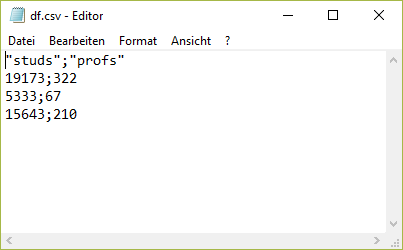
\includegraphics{././pic/102_csvdatei.png}

\begin{tcolorbox}[standard jigsaw,leftrule=.75mm, bottomtitle=1mm, rightrule=.15mm, opacitybacktitle=0.6, toprule=.15mm, titlerule=0mm, toptitle=1mm, colbacktitle=quarto-callout-warning-color!10!white, bottomrule=.15mm, arc=.35mm, coltitle=black, left=2mm, title=\textcolor{quarto-callout-warning-color}{\faExclamationTriangle}\hspace{0.5em}{Warning}, colframe=quarto-callout-warning-color-frame, opacityback=0, colback=white]
Nun wollen wir also eine csv-Datei einlesen, konkret eine reduzierte
Version des bereits in der Vorlesung erwähnten Allbus-Datensatzes für
das Jahr 2016.\footnote{Allbus steht für ``Allgemeine
  Bevölkerungsumfrage der Sozialwissenschaften'' und ist eine
  zweijährlich durchgeführte allgemeine Umfrage, welche repräsentative
  viele Aspekte der politischen und sozialen Einstellungen in
  Deutschland abfragt. Als Studierende können Sie sich sowohl den Allbus
  2016 als auch die Ausgaben für weitere Jahre hier unkompliziert
  herunterladen:
  \url{https://www.gesis.org/allbus/download/download-querschnitte/}}
Sie finden die csv-Datei ``allbus2016\_kompakt.csv'' auf StudIP:
\end{tcolorbox}

Um den Datensatz nun in R zu importieren, sind zwei Schritte notwendig.
Zuerst müssen wir R mitteilen unter welchem Dateipfad der Datensatz zu
finden ist. Der Dateipfad ergibt sich aus der Ordnerstruktur Ihres
Gerätes, so würde der Dateipfad im hier dargestellten Fall
\emph{``C:/Users/Andreas/Dokumente/Statistik/''} lauten:

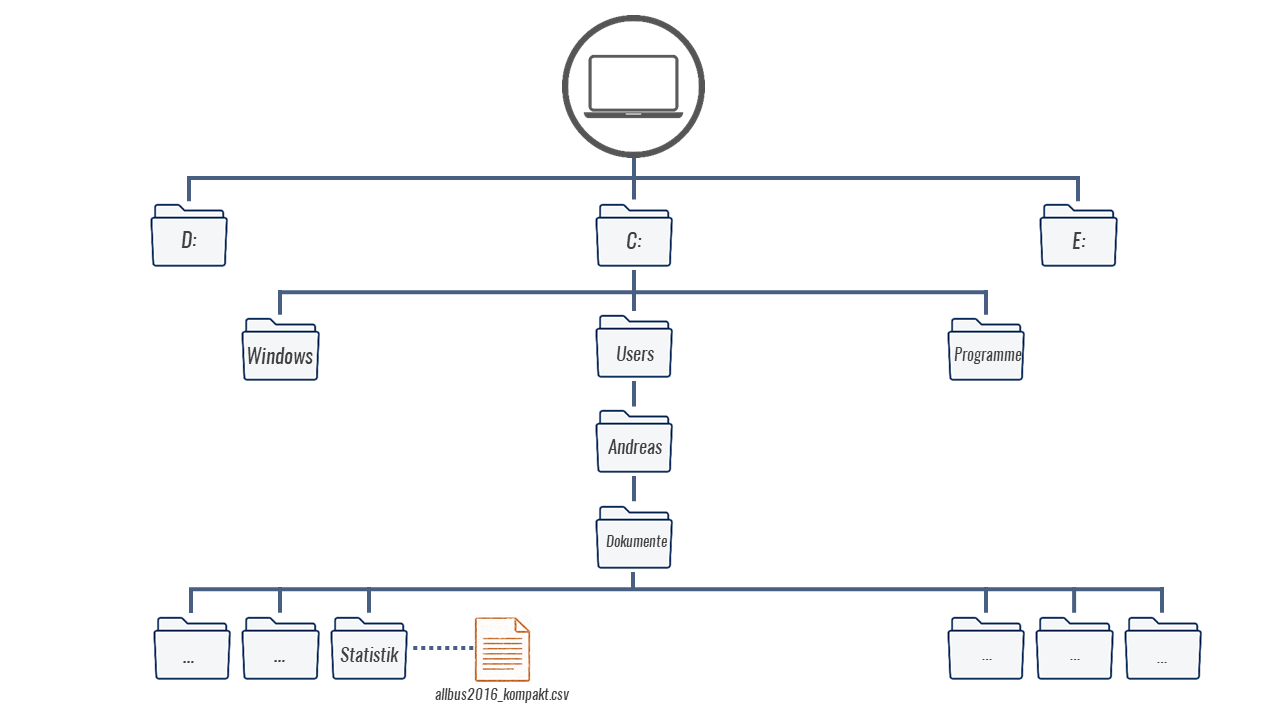
\includegraphics{././pic/102_dateipfad.png}

Natürlich hängt der Dateipfad aber ganz davon ab, wo Sie den Datensatz
gespeichert haben. Um den Pfad des Ordners herauszufinden, klicken Sie
bei Windows in die obere Adresszeile im Explorerfenster, bei Mac finden
Sie den Pfad indem Sie einmal mit der rechten Maustaste auf die Datei
und unter Informationen den Reiter ``Ort'' wählen.

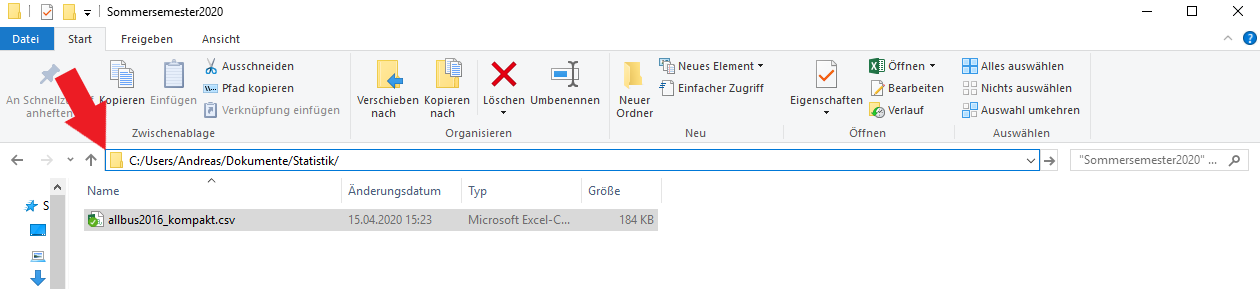
\includegraphics{././pic/102_Dateipfad_Win.png}

Diesen Dateipfad müssen wir also R mitteilen. Dafür gibt es mehrere
Varianten, die einfachste ist \texttt{setwd()}. Wir setzen in die
Klammern den Pfad des Ordners ein, in dem der Allbus-Datensatz
gespeichert ist. Wichtig dabei ist dass Sie ggf. alle
\texttt{\textbackslash{}} durch \texttt{/}ersetzen müssen:

\begin{Shaded}
\begin{Highlighting}[]
\FunctionTok{setwd}\NormalTok{(}\StringTok{"C:/Users/Andreas/Dokumente/Statistik/"}\NormalTok{)}
\end{Highlighting}
\end{Shaded}

Mit \texttt{getwd()} lässt sich überprüfen, ob das funktioniert hat:

\begin{Shaded}
\begin{Highlighting}[]
\FunctionTok{getwd}\NormalTok{()}
\end{Highlighting}
\end{Shaded}

Hier sollte der mit \texttt{setwd()} gesetzte Pfad erscheinen.

Ist das der Fall, können wir den eigentlichen Einlesebefehl
\texttt{read.table} verwenden:

\begin{Shaded}
\begin{Highlighting}[]
\NormalTok{a16 }\OtherTok{\textless{}{-}} \FunctionTok{read.table}\NormalTok{(}\StringTok{"allbus2016\_kompakt.csv"}\NormalTok{, }\AttributeTok{sep =} \StringTok{";"}\NormalTok{, }\AttributeTok{header =}\NormalTok{ T, }\AttributeTok{stringsAsFactors =}\NormalTok{ F)}
\end{Highlighting}
\end{Shaded}

Der Einlesevorgang besteht aus zwei Teilen: zuerst geben wir mit
\texttt{a16} den Namen an, unter dem R den Datensatz ablegt. Nach dem
\texttt{\textless{}-} steht dann der eigentliche Befehl
\texttt{read.table()}, der wiederum mehrere Optionen enthält. Als erstes
geben wir den genauen Datensatznamen an - inklusive der Dateiendung.
Darüber hinaus teilen wir R mit \texttt{sep} mit, dass ; als
Trennzeichen gesetzt wurde und mit \texttt{header\ =\ T} teilen wir R
zudem mit, dass die erste Zeile aus dem Datensatz als Spaltennamen
verwendet werden soll. \texttt{stringsAsFactors\ =\ F} legt fest, dass
Variablen mit Buchstaben (sog. strings) nicht in das Spezialformat
\texttt{factor} überführt werden sollen (warum und was
\texttt{factor}-Variablen sind, besprechen wir später).

Würden hier jetzt einfach \texttt{a16} eintippen bekämen wir den
kompletten Datensatz angezeigt. Für einen Überblick können wir
\texttt{head} verwenden:

\begin{Shaded}
\begin{Highlighting}[]
\FunctionTok{head}\NormalTok{(a16)}
\end{Highlighting}
\end{Shaded}

\begin{verbatim}
  respid eastwest german sex mborn yborn age agec pyborn page pagec di01a educ
1      1        2      1   2     9  1968  47    3    -10  -10   -10  1800    3
2      2        2      1   1     9  1963  52    3    -10  -10   -10  2000    3
3      3        1      1   1     1  1955  61    4    -10  -10   -10  2500    2
4      4        1      1   2     7  1961  54    3    -10  -10   -10   860    2
5      5        1      1   1     1  1945  71    4    -10  -10   -10    -7    5
6      6        1      1   1     8  1967  49    3    -10  -10   -10  2500    3
  mstat gkpol land  inc
1     1     2  160 1800
2     1     7  112 2000
3     1     3   60 2500
4     1     7  111  860
5     1     6   50   -9
6     4     2   30 2500
\end{verbatim}

Mit \texttt{nrow} und \texttt{ncol} können wir kontrollieren, ob das
geklappt hat. Der Datensatz sollte 3490 Zeilen und 17 Spalten haben:

\begin{Shaded}
\begin{Highlighting}[]
\FunctionTok{nrow}\NormalTok{(a16)}
\end{Highlighting}
\end{Shaded}

\begin{verbatim}
[1] 3490
\end{verbatim}

\begin{Shaded}
\begin{Highlighting}[]
\FunctionTok{ncol}\NormalTok{(a16)}
\end{Highlighting}
\end{Shaded}

\begin{verbatim}
[1] 17
\end{verbatim}

Mit \texttt{View(a16)} öffnet sich zudem ein neues Fenster, in dem wir
den gesamten Datensatz ansehen können.

Natürlich können wir wie oben auch aus diesem, viel größeren, Datensatz
Zeilen und Spalten auswählen. Zum Beispiel können wir die Befragten
auswählen, die älter als 87 Jahre alt sind und diese unter
\texttt{senior} ablegen:

\begin{Shaded}
\begin{Highlighting}[]
\NormalTok{senior }\OtherTok{\textless{}{-}}\NormalTok{ a16[a16}\SpecialCharTok{$}\NormalTok{age }\SpecialCharTok{\textgreater{}} \DecValTok{87}\NormalTok{,]}
\end{Highlighting}
\end{Shaded}

Möchten wir die genauen Altersangaben der Befragten aus \texttt{senior}
sehen, können wir die entsprechende Spalte mit \texttt{senior\$age}
aufrufen:

\begin{Shaded}
\begin{Highlighting}[]
\NormalTok{senior}\SpecialCharTok{$}\NormalTok{age}
\end{Highlighting}
\end{Shaded}

\begin{verbatim}
 [1] 88 88 88 90 88 88 91 90 90 88 88 88 88 91 90 89 88 89 91 97 89 88 88 90 93
\end{verbatim}

Außerdem hat \texttt{senior} natürlich deutlich weniger Zeilen als
\texttt{a16}:

\begin{Shaded}
\begin{Highlighting}[]
\FunctionTok{nrow}\NormalTok{(senior)}
\end{Highlighting}
\end{Shaded}

\begin{verbatim}
[1] 25
\end{verbatim}

Wie wir beim Überblick gesehen haben, gibt es aber noch deutlich mehr
Variablen im Allbus als \texttt{age} und nicht alle haben so
aussagekräftige Namen - z.B. \texttt{gkpol}. Um diese Variablennamen und
auch die Bedeutung der Ausprägungen zu verstehen brauchen wir das
Codebuch. In ihm sind alle Variablennamen sowie die Ausprägungen
erläutert. Laden Sie daher auch das Codebuch für den Allbus
(Codebuch\_allbus.pdf) herunter, wir werden es häufig brauchen!

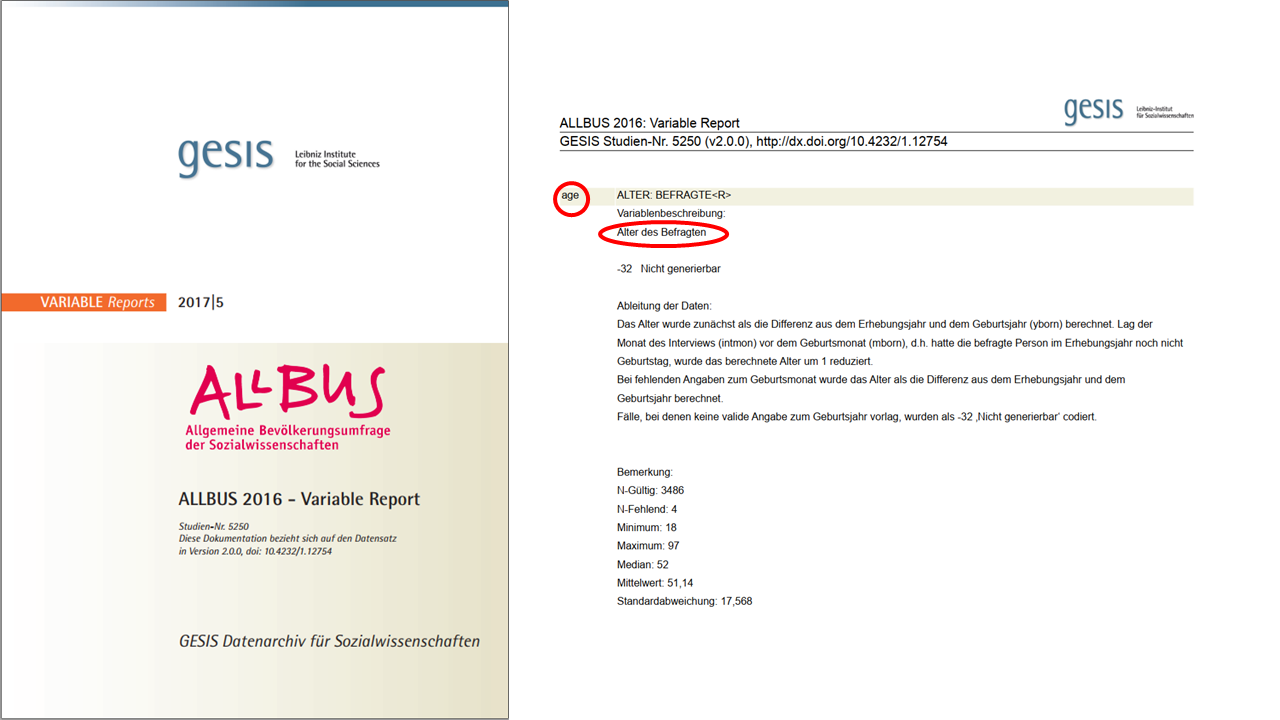
\includegraphics{././pic/102_codebuch_comb.png}

\hypertarget{aufgaben-1}{%
\section{Aufgaben}\label{aufgaben-1}}

\begin{itemize}
\item
  Sie finden in StudIP im Ordner Übungsunterlagen den Allbus 2016 unter
  dem Namen \texttt{allbus2016\_kompakt.csv}. Laden Sie die Datei
  herunter und speichern Sie sie ab. Öffnen Sie die Datei bitte
  \textbf{nicht} direkt mit Excel, auch wenn Ihnen dies wahrscheinlich
  vorgeschlagen wird.
\item
  Laden Sie den Datensatz \texttt{allbus2016\_kompakt.csv} in R und
  legen Sie den Datensatz unter \texttt{a16} ab.
\item
  Nutzen Sie \texttt{head()} und \texttt{View()}, um sich einen
  Überblick über den Datensatz zu verschaffen.
\item
  Wie viele Befagte (Zeilen) enthält der Datensatz?
\item
  Lassen Sie sich die Variablennamen von \texttt{a16} anzeigen!
\item
  Die Variable \texttt{sex} gibt das Geschlecht der Befragten an.
  Welcher Variablentyp ist für die Variable festgelegt, welches
  Skalenniveau hat die Variable?
\item
  Was verbirgt sich hinter der Variable \texttt{gkpol}? Sehen Sie im
  Codebuch nach! Welche Bedeutung hat die Ausprägung 2 für diese
  Variable?
\item
  Welches Skalenniveau hat \texttt{gkpol}?\footnote{Diese Frage ist eine
    inhaltliche, R hilft Ihnen hier nicht weiter.}
\item
  Welcher Variablentyp ist in R für \texttt{gkpol} festgelegt? Ändern
  Sie den Variablentyp.
\item
  Welche Information ist in der Variable \texttt{respid} abgelegt?
\item
  Wie können Sie sich die Zeile anzeigen lassen, welche den/die
  Befragte*n mit der \texttt{respid} 3469 enthält?
\item
  Wie alt ist der/die Befragte mit der \texttt{respid} 3469? Welches
  Geschlecht hat die Person?
\item
  Erstellen Sie eine neue Variable mit dem Alter der Befragten im Jahr
  2020!
\item
  Wählen Sie alle Befragten aus, die nach 1960 geboren wurden legen Sie
  diese Auswahl unter \texttt{nach\_1960} ab.
\item
  Wie viele Spalten hat \texttt{nach\_1960}? Wie viele Zeilen? Nutzen
  Sie für Ihre Antwort die Befehle die wir kennen gelernt haben.
\end{itemize}

\hypertarget{tab}{%
\chapter{Überblick erhalten: Tabellen}\label{tab}}

\begin{Shaded}
\begin{Highlighting}[]
\FunctionTok{table}\NormalTok{(mtcars}\SpecialCharTok{$}\NormalTok{cyl) }
\end{Highlighting}
\end{Shaded}

\begin{verbatim}
 4  6  8 
11  7 14 
\end{verbatim}

\hypertarget{regressionsmodelle}{%
\chapter{Regressionsmodelle}\label{regressionsmodelle}}

\hypertarget{annahmen-checken}{%
\section{Annahmen checken}\label{annahmen-checken}}

\begin{Shaded}
\begin{Highlighting}[]
 \CommentTok{\# install.packages(\textquotesingle{}see\textquotesingle{})}
\FunctionTok{library}\NormalTok{(performance)}
\FunctionTok{data}\NormalTok{(mtcars)}
\NormalTok{mtcars}\SpecialCharTok{$}\NormalTok{gear }\OtherTok{\textless{}{-}} \FunctionTok{factor}\NormalTok{(mtcars}\SpecialCharTok{$}\NormalTok{gear) }\CommentTok{\# }
\NormalTok{m1 }\OtherTok{\textless{}{-}} \FunctionTok{lm}\NormalTok{(mpg }\SpecialCharTok{\textasciitilde{}}\NormalTok{ qsec, mtcars)}
\NormalTok{m2 }\OtherTok{\textless{}{-}} \FunctionTok{lm}\NormalTok{(mpg }\SpecialCharTok{\textasciitilde{}}\NormalTok{ qsec }\SpecialCharTok{+}\NormalTok{ gear, mtcars)}

\FunctionTok{check\_model}\NormalTok{(m2)}
\end{Highlighting}
\end{Shaded}

\begin{figure}[H]

{\centering 
\includegraphics{./09_reg_files/figure-pdf/reg02-1.pdf}

}

\end{figure}

\hypertarget{regressionsmodelle-vergleichen}{%
\section{Regressionsmodelle
vergleichen}\label{regressionsmodelle-vergleichen}}

Mit dem Paket \texttt{\{performance\}} können wir auch einen umfassenden
Modellvergleich bekommen: ::: \{.cell\}

\begin{Shaded}
\begin{Highlighting}[]
\FunctionTok{compare\_performance}\NormalTok{(m1,m2)}
\end{Highlighting}
\end{Shaded}

\begin{verbatim}
# Comparison of Model Performance Indices

Name | Model |     AIC | AIC weights |     BIC | BIC weights |    R2 | R2 (adj.) |  RMSE | Sigma
------------------------------------------------------------------------------------------------
m1   |    lm | 204.588 |     < 0.001 | 208.985 |       0.003 | 0.175 |     0.148 | 5.387 | 5.564
m2   |    lm | 190.061 |       0.999 | 197.390 |       0.997 | 0.538 |     0.488 | 4.033 | 4.312
\end{verbatim}

:::

\hypertarget{summary}{%
\chapter{Summary}\label{summary}}

In summary, this book has no content whatsoever.

\begin{Shaded}
\begin{Highlighting}[]
\DecValTok{1} \SpecialCharTok{+} \DecValTok{1}
\end{Highlighting}
\end{Shaded}

\begin{verbatim}
[1] 2
\end{verbatim}

\hypertarget{references}{%
\chapter*{References}\label{references}}
\addcontentsline{toc}{chapter}{References}

\hypertarget{refs}{}
\begin{CSLReferences}{0}{0}
\end{CSLReferences}

\end{document}
